% Created 2023-01-14 Σαβ 15:21
% Intended LaTeX compiler: pdflatex
\documentclass[11pt]{article}
\usepackage[utf8]{inputenc}
\usepackage[T1]{fontenc}
\usepackage{graphicx}
\usepackage{longtable}
\usepackage{wrapfig}
\usepackage{rotating}
\usepackage[normalem]{ulem}
\usepackage{amsmath}
\usepackage{amssymb}
\usepackage{capt-of}
\usepackage{hyperref}
\usepackage{booktabs}
\usepackage{import}
\usepackage[LGR, T1]{fontenc}
\usepackage[greek, english]{babel}
\usepackage{alphabeta}
\usepackage{esint}
\usepackage{mathtools}
\usepackage{esdiff}
\usepackage{makeidx}
\usepackage{glossaries}
\usepackage{newfloat}
\usepackage{minted}
\usepackage{chemfig}
\usepackage{svg}
\usepackage[a4paper, margin=3cm]{geometry}
\newcommand{\HRule}{\rule{\linewidth}{0.5mm}}
\date{}
\title{Αξιοποίηση Πυρηνόξυλου για Παραγωγή Γλυκερόλης και Κυκλοπεντανόνης}
\hypersetup{
 pdfauthor={Vidianos Giannitsis},
 pdftitle={Αξιοποίηση Πυρηνόξυλου για Παραγωγή Γλυκερόλης και Κυκλοπεντανόνης},
 pdfkeywords={},
 pdfsubject={},
 pdfcreator={Emacs 28.2 (Org mode 9.5.5)}, 
 pdflang={English}}
\makeatletter
\newcommand{\citeprocitem}[2]{\hyper@linkstart{cite}{citeproc_bib_item_#1}#2\hyper@linkend}
\makeatother

\usepackage[notquote]{hanging}
\begin{document}

\renewcommand{\abstractname}{Περίληψη}
\renewcommand{\tablename}{Πίνακας}
\renewcommand{\figurename}{Σχήμα}
\renewcommand\listingscaption{Κώδικας}

\renewcommand{\contentsname}{Περιεχόμενα}
\begin{titlepage}

\begin{center}
  \begin{minipage}{0.15\textwidth}
    \begin{flushleft}
      \includegraphics[width=1\textwidth]{~/Pictures/ntua_logo.png}\\[0.4cm]    
    \end{flushleft}
  \end{minipage}
  \begin{minipage}{0.80\textwidth}
    \textsc{\bfseries \large ΕΘΝΙΚΟ ΜΕΤΣΟΒΙΟ ΠΟΛΥΤΕΧΝΕΙΟ}\\[0.2cm]
    \textsc{\bfseries \large ΣΧΟΛΗ ΧΗΜΙΚΩΝ ΜΗΧΑΝΙΚΩΝ - ΤΟΜΕΑΣ ΙΙ}\\[0.2cm]
    \textsc{\bfseries \normalsize ΕΡΓΑΣΤΗΡΙΟ ΣΧΕΔΙΑΣΜΟΥ ΚΑΙ ΑΝΑΛΥΣΗΣ ΔΙΕΡΓΑΣΙΩΝ}\\[0.2cm]
  \end{minipage}
  \\[1.5cm]

  \Large Εργασία Μαθήματος <<Σχεδιασμός Διεργασιών>>\\[1.5cm]
  \HRule \\[0.4cm]
  { \textsc{\huge \bfseries Αξιοποίηση Πυρηνόξυλου για Παραγωγή Γλυκερόλης και Κυκλοπεντανόνης}}\\[0.4cm]
  \HRule \\[3cm]

  \begin{minipage}{0.4\textwidth}
    \begin{flushleft} \large
      \emph{Συγγραφείς:}\\
      Βιδιάνος Γιαννίτσης\\
      Αριστοτέλης Αργυρόπουλος\\
      Διονύσης Γιαννάτος\\
      Θεωφανώ Αντωνία Πόταρη\\
      Στυλιανή Σταύρου\\
      Έλλη Πούτα
    \end{flushleft}
  \end{minipage}
  \begin{minipage}{0.4\textwidth}
    \begin{flushright} \large
      \emph{Αριθμοί Μητρώου:}\\
      ch19113\\
      ch19114\\
      ch19074\\
      ch19555\\
      ch19606\\
      ch19534
    \end{flushright}
  \end{minipage}\\[1cm]
  \HRule \\[2cm]

  \vfill
  {\large Αθήνα, 2022}
\end{center}

\end{titlepage}

\tableofcontents
\pagebreak

\section{Εισαγωγή}
\label{sec:org79c2c53}
Σκοπός της εργασίας αυτής είναι η αξιοποίηση του πυρηνόξυλου, δηλαδή του ξυλώδους κομματιού του πυρήνα της ελιάς, για την παραγωγή γλυκερόλης και κυκλοπεντανόνης, οι οποίες είναι δύο χρήσιμες οργανικές ενώσεις.

H κυκλοπεντανόνη είναι μία κυκλική οργανική χημική ένωση με μοριακό
τύπο C\textsubscript{5}H\textsubscript{8}O και ανήκει στη κατηγορία των οργανικών ενώσεων που
ονομάζονται κετόνες. Συγκεκριμένα, αποτελείται δομικά
από έναν πενταμελή δακτύλιο που περιέχει τη λειτουργική ομάδα των
κετονών. Η φυσική της μορφή είναι ένα άχρωμα υγρό με χαρακτηριστική οσμή
παραπλήσια με μέντα. Η επιθυμία παραγωγής της κυκλοπεντανόνης προέρχεται
από το γεγονός ότι είναι βασικό χημικό ενδιάμεσο προϊόν τόσο στη
φαρμακοβιομηχανία όσο και στην κατασκευή αρωμάτων. Επίσης, είναι
απαραίτητο συστατικό για την κατασκευή εντομοκτόνων και προϊόντων από
καουτσούκ \textsuperscript{\citeprocitem{1}{1}}. Ακόμη, χρησιμοποιείται ευρέως ως διαλύτης, για αυτό είναι ενδιαφέρουσα η παραγωγή από πράσινη πρώτη ύλη.

Η κυκλοπεντανόνη παράγεται ως προιόν της φουρφουράλης, η οποία είναι ένα εξαιρετικά χρήσιμο χημικό ενδιάμεσο \textsuperscript{\citeprocitem{2}{2}} μέσω μίας αντίδρασης υδρογόνωσης. Η φουρφουράλη με τη σειρά της παράγεται από το ημικυτταρινικό κλάσμα της βιομάζας και συγκεκριμένα μέσω της όξινης καταλυτικής αφυδάτωσης της ξυλόζης.

Η γλυκερόλη είναι η απλούστερη δυνατή τριόλη, δηλαδή μία οργανική ένωση με τρείς αλκοολομάδες. Έχει μοριακό τύπο \(C_3H_8O_3\). Είναι μία ένωση η οποία έχει ευρεία χρήση σε φαρμακοβιομηχανίες, ιδιαίτερα αν ανακτηθεί σε υψηλή καθαρότητα (της τάξης του \(99.9 \%\)). Επίσης, μπορεί να χρησιμοποιηθεί ως πρώτη ύλη για την παραγωγή πολλών χρήσιμων προιόντων σε ένα πλαίσιο βιοδιυλιστηρίου, για αυτό είναι πολύ ενδιαφέρουσα η μελέτη της παραγωγής γλυκερόλης από βιομάζα, η οποία έχει υψηλή καθαρότητα και διατίθεται σε χαμηλή τιμή \textsuperscript{\citeprocitem{3}{3}} .

Η γλυκερόλη είναι μία ένωση η οποία παράγεται σε μεγάλες ποσότητες από την βιομηχανία του βιοντίζελ με πράσινο τρόπο. Το βιοντίζελ είναι ένα σημαντικό βιοκαύσιμο που έχει αρχίσει να χρησιμοποιείται ευρέως τα τελευταία χρόνια. Λόγω της μεγάλης περίσσειας γλυκερόλης που παράγεται από την διεργασία αυτή, έχει υποτιμηθεί σημαντικά η αξία της. Όμως, η διεργασία αυτή παράγει ακατέργαστη γλυκερόλη αρκετά χαμηλής καθαρότητας, ο καθαρισμός της οποίας είναι πολύ ακριβός και τυπικά δεν συμφέρει την εγκατάσταση \textsuperscript{\citeprocitem{4}{4}–\citeprocitem{6}{6}} . Σε εφαρμογές που απαιτούν πολύ υψηλή καθαρότητα, τυπικά χρησιμοποιείται συνθετικά παραγόμενη γλυκερόλη η οποία παράγεται από προπυλένιο. Για αυτό, υπάρχει αρκετό ενδιαφέρον στην εύρεση μίας διεργασίας η οποία θα παράξει απευθείας γλυκερόλη από βιομάζα σε υψηλή καθαρότητα. Μία τέτοια διεργασία είχε χρησιμοποιήθει στον πρώτο παγκόσμιο πόλεμο για την παραγωγή νιτρογλυκερίνης ως εκρηκτικό, με τον μικροοργανισμό S. cerevisiae. Όμως, σε μεταγενέστερες μελέτες αυτής της αντίδρασης, βρέθηκε πως η απόδοση της διεργασίας αυτής είναι πολύ χαμηλή και δεν αξίζει οικονομικά η κλιμάκωση μίας τέτοιας διεργασίας \textsuperscript{\citeprocitem{7}{7},\citeprocitem{8}{8}} .

Για αυτό, στην παρούσα μελέτη ασχοληθήκαμε με οσμοφιλικές ζύμες οι οποίες έχουν πολύ υψηλότερη απόδοση στην παραγωγή πολυολών και συγκεκριμένα με την ζύμη Candida glycerinogenes η οποία είναι ιδαίτερα αποδοτική στην παραγωγή γλυκερόλης \textsuperscript{\citeprocitem{8}{8}–\citeprocitem{10}{10}} .

\subsection{Δυναμικότητα Εργοστασίου σε πρώτη ύλη και προιόντα}
\label{sec:orgb4d5b9d}
Η προσομοίωση της διεργασίας έγινε θεωρόντας ως τροφοδοσία 200000 tn/y πυρηνόξυλο, η οποία θεωρήθηκε η δυναμικότητα του εργοστασίου. Με βάση την βιβλιογραφία \textsuperscript{\citeprocitem{11}{11}–\citeprocitem{14}{14}} αυτό σημαίνει πως η θεωρητική ποσότητα κυτταρίνης η οποία υπάρχει σε αυτό είναι 74000 tn/y ενώ η ποσότητα ημικυτταρίνης είναι 53000 tn/y. Από αυτά, μπορεί να διαπιστωθεί μία ψευδοαπόδοση των διεργασιών μετατροπής της κυτταρίνης σε γλυκερόλη και της ημικυτταρίνης σε κυκλοπεντανόνη.

Από τις ποσότητες αυτές, ανακτήθηκαν 27764 tn/y γλυκόζη και 23307 tn/y ξυλόζη με βάση την προκατεργασία που υπέστη η βιομάζα. Η προκατεργασία αυτή βασίστηκε στην έκρηξη ατμού, η οποία είναι μία θερμική μέθοδος στην οποία υπάρχουν σημαντικές απώλειες λόγω θερμικής διάσπασης των πολυμερών. Επίσης, παρότι είναι τα βασικά συστατικά των δύο πολυμερών, δεν μπορεί να ανακτηθεί όλη η ποσότητα τους σε μία τυπική διεργασία.

Τα τελικά μας προιόντα είναι σε ποσότητες 10437 tn/y γλυκερόλη 17765 tn/y κυκλοπεντανόνη, λαμβάνοντας υπόψην όλες τις φυσικές και χημικές διεργασίες που χρησιμοποιήθηκαν, καθώς σε όλες υπάρχει μία απώλεια. Η γλυκερόλη έχει μία σχετικά χαμηλή απόδοση (μόνο το \(37.6 \%\) της γλυκόζης μετατρέπεται σε γλυκερόλης) λόγω της βιοχημικής διεργασίας που ακολουθήθηκε για την παραγωγή της. Είναι γνωστό πως κατά την ανάπτυξη ενός μικροοργανισμού, η πηγή άνθρακα του - δηλαδή η γλυκόζη - δεν καταναλώνεται μόνο για την παραγωγή χρήσιμων προιόντων, για αυτό δεν αναμένεται πολύ υψηλή απόδοση σε προιόν. Βέβαια, με βάση την βιβλιογραφία είναι από τις καλύτερες δυνατές αποδόσεις που μπορούμε να πετύχουμε. Η κυκλοπεντανόνη, έχει μία αρκετά καλύτερη απόδοση. Το \(77.8 \%\) της ξυλόζης μετατρέπεται σε κυκλοπεντανόνη, διότι για την μετατροπή αυτή δεν απαιτείται βιοχημική διεργασία, άρα οι αντιδραστήρες μπορούν να λειτουργούν σε πολύ υψηλές μετατροπές.

\subsection{Οικονομικό Δυναμικό της Διεργασίας}
\label{sec:org4a33da0}
Πριν γίνει όμως οποιαδήποτε επένδυση, είναι πολύ σημαντικό να υπάρχει μία εικόνα του οικονομικού δυναμικού της διεργασίας. Το οικονομικό δυναμικό είναι μία πρώτη εικόνα των οικονομικών της διεργασίας, λαμβάνοντας υπόψην μόνο το κόστος των πρώτων υλών και τα έσοδα της διεργασίας. Για να αξίζει μία διεργασία, αναμένεται πως το ετήσιο κέρδος της θα είναι αρκετά υψηλό. Στην ολοκληρώμενη οικονομική ανάλυση της διεργασίας, πρέπει να ληφθεί υπόψην και το πάγιο κόστος του εξοπλισμού. Όμως, αυτή η ανάλυση θα γίνει σε μεταγενέστερο στάδιο.

Το θετικό με μία τέτοια διεργασία, η οποία διαχειρίζεται απόβλητα ως πρώτη ύλη είναι ότι οι πρώτες ύλες που απαιτούνται πέραν αυτόν που υπάρχουν ήδη από την βιομάζα είναι λίγες. Για αυτό, το οικονομικό δυναμικό τέτοιων διεργασιών είναι τυπικά αρκετά υψηλό. Στην περίπτωση μας, το μόνο κόστος που υπάρχει πέραν της βιομάζας είναι οι θρεπτικές ουσίες που απαιτούνται για την ανάπτυξη του μικροοργανισμού που παράγει την γλυκερόλη και το υδρογόνο που χρησιμοποιείται για την παραγωγή της κυκλοπεντανόνης, ενώ ως κέρδος υπάρχει η πώληση των δύο προιόντων.

Από την πλευρά της γλυκερόλης άρα, η πώληση της γλυκερόλης επιφέρει κέρδος 8.35 εκατομμύρια ευρώ τον χρόνο ενώ οι θρεπτικές ουσίες που χρειάζονται (ουρία και corn steep liquor) έχουν κόστος 327 χιλιάδες ευρώ. Άρα, το οικονομικό δυναμικό της διεργασίας αυτής είναι περίπου 8 εκατομμύρια ευρώ το έτος. Παρακάτω υπάρχουν και οι πηγές από τις οποίες βρέθηκαν αυτά:

\href{https://www.selinawamucii.com/insights/prices/united-states-of-america/glycerol/}{Γλυκερόλη: 721 ευρώ ανά τόνο}

\href{https://www.indiamart.com/proddetail/corn-steep-liquor-15744963191.html}{Corn Steep Liquor: 360 ευρώ ανά τόνο}

\href{https://tradingeconomics.com/commodity/urea}{Ουρία: 638 ευρώ ανά τόνο}

Από την πλευρά της κυκλοπεντανόνης, η πώληση της επιφέρει κέρδος 92.8 εκατομμύρια το έτος ενώ το υδρογόνο κοστίζει 2.6 εκατομμύρια το έτος με βάση τις τιμές τους στην αγορά. Άρα έχει ένα οικονομικό δυναμικό 90.2 εκατομμύρια ευρώ το έτος. Παρακάτω υπάρχουν και οι πηγές από τις οποίες βρέθηκαν αυτά:

\href{https://www.sgh2energy.com/economics}{Υδρογόνο: 2 ευρώ ανά κίλο}

\href{https://dir.indiamart.com/impcat/cyclopentanone.html}{Κυκλοπεντανόνη: 5.12 ευρώ ανά κιλό}

Ακόμη, υπάρχει η σκέψη ότι μπορεί το υδρογόνο να παραχθεί με αναμόρφωση της λιγνίνης η οποία είναι διαθέσιμη σε μεγάλη ποσότητα, παράγοντας έτσι υδρογόνο μέσα στη διεργασία και εξαλείφοντας το κόστος αυτό. 

Άρα, το συνολικό οικονομικό δυναμικό της διεργασίας είναι 98.2 εκατομμύρια ευρώ το έτος, το οποίο σημαίνει ότι υπάρχει αρκετό διάστημα για δαπάνες σε ηλεκτρική ενέργεια, βοηθητικές παροχές και εξοπλισμό.

\section{Μέθοδος Ανάλυσης της Συνολικής Διεργασίας}
\label{sec:org62648cf}
Μία συχνή τακτική για την παρουσίαση μεγάλων διεργασιών όπου το συνολικό διάγραμμα ροής που προκύπτει είναι πολύ μεγάλο για να παρουσιαστεί σε μία εικόνα είναι οι διεργασίες να χωρίζονται σε blocks αριθμημένα με τη λογική 100, 200, 300 κλπ. Έτσι, τα διαγράμματα ροής που παρουσιάζονται είναι μικρά και εύκολα στην κατανόηση, αλλά δεν χαλάει η λογική συνέχεια επειδή μπορεί να αναφερθεί ότι η τροφοδοσία του ενός block είναι προιόν ενός άλλου. Καθώς η διεργασία που έχουμε σχεδιάσει για το μάθημα είναι πολύ μεγάλη, θα ακολουθηθεί αυτή η προσέγγιση.

Η διεργασία μας έχει χωριστεί σε 7 blocks. Τo block 100 αφορά την προκατεργασία της βιομάζας ώστε να κλασματοποιηθεί σε κυτταρίνη, ημικυτταρίνη και λιγνίνη, με βασικότερη διεργασία αυτήν της έκρηξης ατμού. Το block 200 αφορά την μετατροπή της κυτταρίνης σε γλυκόζη, ώστε η γλυκόζη αυτή να οδηγηθεί στο block 400 στο οποίο παράγεται η γλυκερόλη στον βιοαντιδραστήρα όπου αναπτύσσεται ο μικροοργανισμός Candida glycerinogenes. Tα προιόντα του αντιδραστήρα αυτού οδηγούνται στο block 500 όπου καθαρίζεται η γλυκερόλη για να είναι στην επιθυμητή καθαρότητα.

To block 300 που δεν αναφέρθηκε είναι το block αξιοποίησης της λιγνίνης. Αποτελεί έναν λέβητα καύσης της λιγνίνης για παραγωγή ατμού υψηλής πίεσης ο οποίος μπορεί να χρησιμοποιηθεί ως θερμαντικό μέσο αλλά και για ηλεκτροπαραγωγή σε διάφορα σημεία της εγκατάστασης.

Τέλος, τα block 600 και 700 είναι για την εκμετάλλευση της ξυλόζης. Στο block 600 η ξυλόζη αφυδατώνεται προς παραγωγή φουρφουράλης, η οποία είναι το ενδιάμεσο προιόν από το οποίο παράγεται η κυκλοπεντανόνη, ενώ στο block 700 γίνονται οι διαχωρισμοί για την ανάκτηση καθαρής κυκλοπεντανόνης.

Ενδεικτικά, παρατίθεται ένα block diagram που δείχνει τις εισόδους και εξόδους από το κάθε block, ενώ παρακάτω θα ακολουθήσει η ανάλυση αυτών.

\begin{figure}[htbp]
\centering
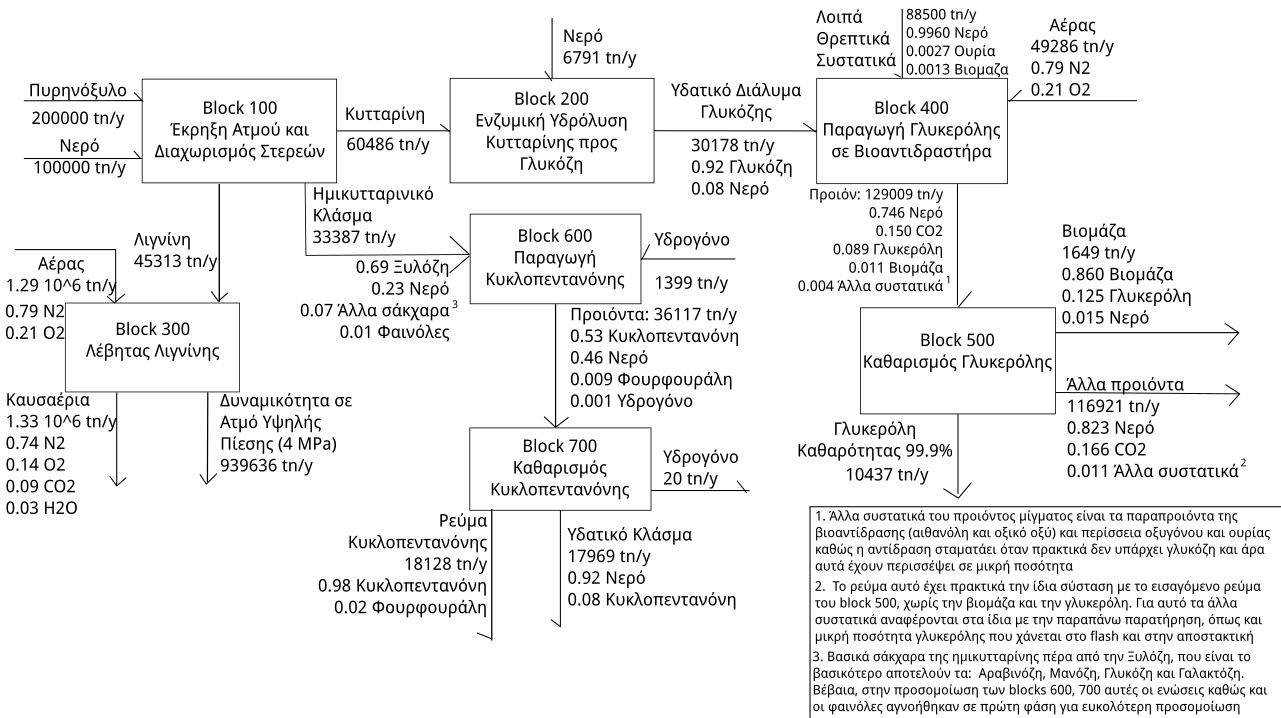
\includegraphics[width=.9\linewidth]{/home/vidianos/Documents/7o_εξάμηνο/Σχεδιασμός_Ι/Project/git_repo/Diagrams/block_diagram.png}
\caption{Block Diagram της Διεργασίας}
\end{figure}

\section{Ανάλυση του block 100 - Έκρηξη Ατμού και Κλασματοποίηση Βιομάζας}
\label{sec:org775d14b}

\subsection{Διάγραμμα ροής και επεξήγηση}
\label{sec:orgc4fc6cf}
\begin{figure}[htbp]
\centering
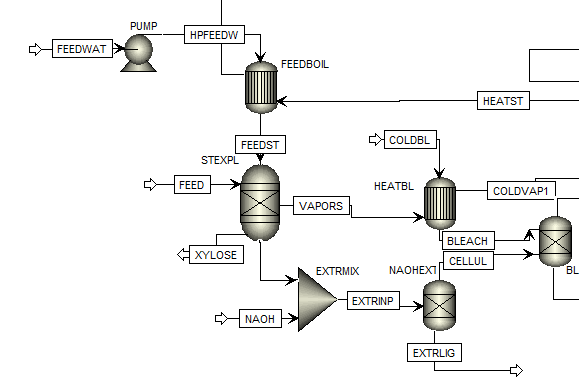
\includegraphics[width=.9\linewidth]{/home/vidianos/Documents/7o_εξάμηνο/Σχεδιασμός_Ι/Project/git_repo/Final_exam_files/Block_100_-_Steam_Explosion/2023-01-10_18-30-22_screenshot.png}
\caption{Διάγραμμα ροής του block 100}
\end{figure}

Στο block 100 γίνεται η αρχική τροφοδοσία της διεργασίας (πυρηνόξυλο) και η κλασματοποίηση του στα 3 βασικά του στοιχεία, την κυτταρίνη, την ημικυτταρίνη και την λιγνίνη. Στο διάγραμμα ροής φαίνεται η παραγωγή ατμού υψηλής πίεσης ο οποίος οδηγείται μαζί με το πυρηνόξυλο στην διεργασία της έκρηξης ατμού. Ο ατμός αυτός παράγεται χρησιμοποιώντας τον ατμό υψηλής πίεσης που παράγεται στον λέβητα της εγκατάστασης (block 300). Από την έκρηξη ατμού (steam explosion) βγαίνουν 3 ρεύματα. Το ημικυτταρινικό κλάσμα με κύριο συστατικό την ξυλόζη (XYLOSE στο διάγραμμα), το στερεό κλάσμα της κυτταρίνης και της λιγνίνης και οι ατμοί οι οποίοι οφείλονται κυρίως σε ότι διασπάστηκε θερμικά και απελευθερώθηκε ως υδρατμοί, διοξείδιο του άνθρακα και άζωτο.

Έπειτα, τα στερεά αναμιγνύονται με υδατικό διάλυμα NaOH και οδηγούνται σε μία διάταξη εκχύλισης στερεού-υγρού στην οποία απομακρύνεται μεγάλο ποσοστό της λιγνίνης. Επειδή δεν απομακρύνεται όλη όμως και η ύπαρξη της στην τροφοδοσία του block 200 μειώνει την ταχύτητα καθώς και την απόδοση της διεργασίας, ακολουθεί και ένα bleacher με NaClO το οποίο απομακρύνει όλη την ποσότητα λιγνίνης.

Μία παράβλεψη που έχει γίνει είναι ότι αν δεν ψυχθεί το ρεύμα των στερεών μετά την έκρηξη ατμού, κατά την ανάμιξη του με το υδατικό διάλυμα, μπορεί αυτό να εξατμιστεί, με αποτέλεσμα να μην έχουμε ακριβώς ανάμιξη υγρού-στερεού, αλλά στερεού-αερίου. Για αυτό, πρέπει να ψυχθεί αυτό το ρεύμα. Επίσης, το ρεύμα αυτό καταλήγει μετά από μερικές διεργασίες στο block 200 όπου ψύχεται για να μπεί στον αντιδραστήρα της ενζυμικής υδρόλυσης. Άρα, θα ήταν καλύτερη ίδεα να υπάρχει εδώ ένας ψυκτήρας, το οποίο όμως δεν έχει διορθωθεί λόγω χρόνου.

\subsection{Σχεδιαστικές Επιλογές}
\label{sec:org837ea86}
Η βασικότερη σχεδιαστική επιλογή του block 100 αφορά την έκρηξη ατμού και συγκεκριμένα τον ατμό που χρησιμοποιείται σε αυτήν. Στην βιβλιογραφία, βρέθηκε μία εκτενή λίστα πειραμάτων έκρηξης ατμού σε πυρηνόξυλο για διαφορετικές συνθήκες, αναφέροντας σε κάθε περίπτωση τα yields της διεργασίας \textsuperscript{\citeprocitem{15}{15}} . Συγκρίνοντας τις επιλογές με σκοπό την μεγιστοποίηση της γλυκόζης και ξυλόζης που μπορούν να παραχθούν σε σχέση με την αρχική σύσταση του πυρηνόξυλου σε κυτταρίνη και ημικυτταρίνη, αποφασίστηκε πως η χρήση υπέρθερμου ατμού στα 26 bar και 232 \(^oC\) είναι η ιδανική. Άλλη σημαντική σχεδιαστική επιλογή είναι οι διαχωρισμοί που θα χρησιμοποιηθούν. Η εκχύλιση με υδατικό διάλυμα NaOH είναι μία άρκετά κλασσική διεργασία για τον διαχωρισμό της λιγνίνης από την κυτταρίνης, αλλά δεν μπορεί να απομακρύνει όλη την λιγνίνη με αποτέλεσμα να περισσεύει αρκετή στο ρεύμα της κυτταρίνης \textsuperscript{\citeprocitem{13}{13},\citeprocitem{15}{15}} .

Η σχεδιαστική επιλογή έγκειται στο αν θέλουμε να χρησιμοποιήσουμε αυτό το ρεύμα όπου ξέρουμε ότι η λιγνινή θα δράσει ανασχετικά για τις κυτταρινάσες κατά την υδρόλυση της κυτταρίνης αλλά δεν θα έχει τόσο σημαντική επίδραση εφόσον διαχωρίστηκε σε καλό βαθμό ή αν θέλουμε να κάνουμε ένα παραπάνω βήμα ώστε να απομακρύνουμε όλη την λιγνίνη και να πετύχουμε την μέγιστη δυνατή απόδοση. Το επιπλέον βήμα είναι ένα στάδιο bleaching με ελαφρώς όξινο (με οξικό οξύ) υδατικό διάλυμα NaClO\textsubscript{2}. Με βάση την σχετική βιβλιογραφία, η διεργασία αυτή διώχνει όλη την υπολοιπόμενη λιγνίνη με αποτέλεσμα να έχουμε ένα καθαρό ρεύμα κυτταρίνης \textsuperscript{\citeprocitem{13}{13},\citeprocitem{16}{16}} .

Επίσης βέβαια, έχει σημασία και τι ποσότητα χρειάζεται από τα αντιδραστήρια αυτά για την διεργασία. Γενικά και τα δύο χρειάζονται σχετικά μικρή ποσότητα. Για την εκχύλιση επιλέχθηκε μία παροχή 25 L/min ώστε η μολαρική παροχή του να είναι ίδιας τάξης μεγέθους με αυτήν των στερεών. Το NaOH προτείνεται να είναι της τάξης του \(2 \% \frac{w}{w}\) \textsuperscript{\citeprocitem{15}{15}}. Με παρόμοιο κριτήριο, στο bleaching θα χρησιμοποιηθεί ένα κυβικό μέτρο νερό. Για να πετύχουμε την σύσταση που αναφέρεται στην βιβλιογραφία, σε αυτό θα προστεθούν 20.5 kg NaClO\textsubscript{2} και 6.96 g Οξικό οξύ και το μίγμα θα θερμανθεί στους 70 \(^oC\) (χρησιμοποιόντας την περίσσεια θερμική ενέργεια των ρευμάτων του steam explosion) \textsuperscript{\citeprocitem{16}{16}}.

\subsection{Υπολογισμοί}
\label{sec:org91916d4}
Το σημαντικότερο κομμάτι των υπολογισμών είναι τα ισοζύγια μάζας που απαιτούνται για την διεργασία της έκρηξης ατμού. Εφόσον δεν μπορούμε να προσομοιώσουμε ακριβώς την έκρηξη ατμού στο Aspen, την θεωρήσαμε μία αντίδραση με γνωστά yields, τα οποία μπορούν να υπολογιστούν με την βοήθεια της βιβλιογραφίας \textsuperscript{\citeprocitem{15}{15}} . Έτσι, μπορεί να προσομοιωθεί ως ένας απλός αντιδραστήρας RYield. Παρακάτω παρατίθεται ο πίνακας των yields που υπολογίστηκαν ενώ για περισσότερες λεπτομέρειες υπάρχει το παράρτημα Α και το \href{https://github.com/Vidianos-Giannitsis/Process-Design/blob/master/Calculations/mass\_balances.ods}{αρχείο με τους υπολογισμούς}.

\begin{table}[htbp]
\caption{Yields του Steam Explosion}
\centering
\begin{tabular}{lrr}
Ένωση & Ποσότητα (tn/y) & Yield\\
\hline
Σύνολο & 300000 & 1\\
Κυτταρίνη & 60486 & 0.202\\
Λιγνίνη & 45314 & 0.151\\
Ξυλόζη & 23307 & 0.078\\
Άλλα σάκχαρα & 2887 & 0.009\\
Φαινόλες & 1285 & 0.004\\
Νερό & 138548 & 0.462\\
CO2 & 27385 & 0.091\\
N2 & 788 & 0.003\\
\end{tabular}
\end{table}

Η κυτταρίνη και η λιγνίνη είναι προφανώς βασικά κομμάτια του πυρηνόξυλου. Το ημικυτταρινικό κλάσμα τώρα είναι το υδατοδιαλυτό και όπως διαλύεται ακολουθεί και μία διεργασία αυτουδρόλυσης. Άρα το βρίσκουμε διαλυμένο στην μορφή ενός μίγματος ξυλόζης, μαζί με άλλες ζάχαρες όπως η αραβινόζη, η γαλακτόζη, η μανόζη και η γλυκόζη, φαινόλες και αρκετό νερό. Έπειτα, τα CO\textsubscript{2} και N\textsubscript{2} που παράγονται είναι από την θερμική διάσπαση της βιομάζας. Ένα κομμάτι της βιομάζας θεωρούμε ότι διασπάστηκε θερμικά καθώς το υγρό και το στερεό κλάσμα δεν είναι ίσα με την αρχική τροφοδοσία. Ο άνθρακας που διασπάστηκε θεωρούμε πως έγινε CO\textsubscript{2}, η υγρασία που υπήρχε στο πυρηνόξυλο θεωρούμε ότι απελευθερώθηκε σε ελεύθερη μορφή και τέλος, επειδή η κυτταρίνη και η λιγνίνη δεν περιέχουν άζωτο, ότι άζωτο είχε το πυρηνόξυλο θεωρούμε ότι απελευθερώθηκε ως ελεύθερο άζωτο.

\subsection{Προσομοιώσεις στο Aspen}
\label{sec:org966d25e}
Το μοντέλο που χρησιμοποιήθηκε στις περισσότερες διεργασίες είναι το μοντέλο SRK. Η καταστατική εξίσωση SRK είναι μία πολύ καλή καταστατική εξίσωση για συστήματα σε υψηλή πίεση. Βέβαια, στην διεργασία του bleaching, εισάγεται στον διαχωρισμό οξικό οξύ. Το οξικό οξύ ως μικρό οργανικό οξύ έχει την ιδιαιτερότητα να μπορεί να σχηματίσει δεσμούς υδρογόνου στην αέρια φάση ακόμη και σε χαμηλές πιέσεις. Τυπικά, για συστήματα με οργανικά οξέα προτείνεται η εξίσωση NRTL-HOC για να περιγράψει κατάλληλα την συμπεριφορά τους.

Το ρεύμα εισόδου της διεργασίας εδώ είναι το πυρηνόξυλο. Το πυρηνόξυλο είναι ένα υλικό το οποίο δεν υπάρχει στο Aspen. Μπορεί όμως να οριστεί ως non-conventional component αν ξέρουμε το proximate και ultimate analysis του. Αυτά φαίνονται στους δύο παρακάτω πίνακες.

\begin{table}[htbp]
\caption{Ultimate Analysis του πυρηνόξυλου}
\centering
\begin{tabular}{lr}
Στοιχείο & Τιμή\\
\hline
Άνθρακας & 48.83\\
Οξυγόνο & 43.48\\
Υδρογόνο & 6.23\\
Άζωτο & 0.36\\
Τέφρα & 1.1\\
\end{tabular}
\end{table}

\begin{table}[htbp]
\caption{Proximate Analysis του πυρηνόξυλου}
\centering
\begin{tabular}{lr}
Στοιχείο & Τιμή\\
\hline
Υγρασία & 8.8\\
Fixed Carbon & 16.2\\
Volatile Matter & 72.7\\
Ash & 2.3\\
\end{tabular}
\end{table}

Έπειτα, η διεργασία του steam explosion, παρόλο που είναι μία φυσική διεργασία που σπάει το πυρηνόξυλο στα συστατικά του, πρέπει να προσομοιωθεί ως αντιδραστήρας. Αλλά επειδή δεν ορίζεται στοιχειομετρία για αυτόν, ορίστηκε ως RYield όπως αναφέρθηκε και παραπάνω.

Αξίζει βέβαια να γίνει και μία αναφορά στο πως προσομοιώθηκαν η κυτταρίνη και η λιγνίνη στον αντιδραστήρα. Πρακτικά, ακολουθήθηκε μία μεθοδολογία που βρέθηκε βιβλιογραφικά \textsuperscript{\citeprocitem{17}{17}} η οποία αναφέρει πως μπορούμε να ορίσουμε τα συστατικά ως conventional solids με μοριακούς τύπος \(C_6H_{10}O_5\) και \(C_{7.3}H_{13.9}O_{1.3}\) για την κυτταρίνη και την λιγνίνη αντίστοιχα. Περισσότερες λεπτομέρειες για την προσομοίωση αυτή υπάρχουν στο παράρτημα B.

Έχοντας αναφέρει αυτά, το τελευταίο ζήτημα της προσομοίωσης αυτής είναι οι δύο διαχωρισμοί των στερεών. Αποφασίστηκε πως θα ήταν δύσκολο ή και αδύνατον να οριστούν επαρκείς ιδιότητες για να καταλάβει το Aspen την αλληλεπίδραση της λιγνίνης με τα διαλύματα NaOH και NaClO\textsubscript{2} για αυτό, οι δύο διαχωρισμοί αυτοί ορίστηκαν σε ένα απλό Separator στο οποίο ορίζεται ακριβώς τι γίνεται. Στο πρώτο ορίζουμε το κυτταρινικό ρεύμα με την γνωστή ποσότητα λιγνίνης που περιέχει, ενώ στο δεύτερο ορίζουμε ότι το ρεύμα της λιγνίνης περιέχει το \(100 \%\) της περιεχόμενης λιγνίνης.

\section{Ανάλυση του Block 200 - Παραγωγή Γλυκόζης}
\label{sec:org09758ff}

\subsection{Διάγραμμα ροής και επεξήγηση}
\label{sec:orga80de86}
\begin{figure}[htbp]
\centering
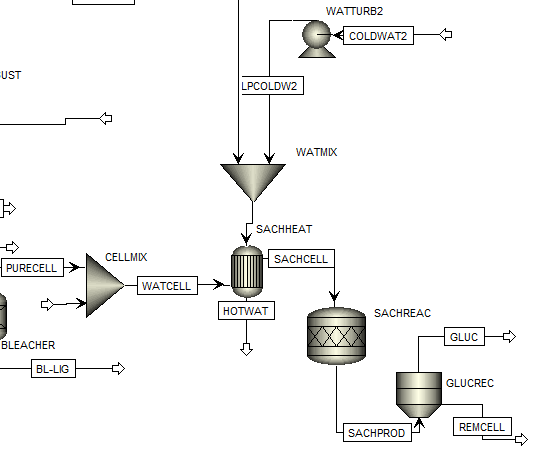
\includegraphics[width=300px]{/home/vidianos/Documents/7o_εξάμηνο/Σχεδιασμός_Ι/Project/git_repo/Final_exam_files/Block_200_-_Παραγωγή_Γλυκόζης/2023-01-10_18-39-54_screenshot.png}
\caption{Διάγραμμα Ροής του block 200}
\end{figure}

Στην παραπάνω εικόνα είναι εμφανής η διεργασία ψύξης και σακχαροποίησης
της κυτταρίνης σε γλυκόζη. Ο εναλλάκτης θερμότητας ψύχει την κυτταρίνη
στους 50 βαθμούς Κελσίου από τους 200 που προκύπτει από την διεργασία
έκρηξης ατμού, ο οποίος αποτυπώνεται στο Block 100. Αξίζει να αναφερθεί πως στην πραγματικότητα, η ψύξη αυτή πρέπει να γίνει μετά την έκρηξη ατμού στο block 100. Όμως, αυτό διαπιστώθηκε αργότερα για αυτό δεν έχει αποτυπωθεί ακόμη στο Aspen.

Έπειτα, η κυτταρίνη τροφοδοτείται σε έναν αντιδραστήρα, ο οποίος αντιπροσωπεύεται στο Aspen ως αντιδραστήρας RYield, και ύστερα τροφοδοτείται σε φυγόκεντρο για τον
διαχωρισμό της στερεής κυτταρίνης από το διάλυμα γλυκόζης, το οποίο
κατευθύνεται στο Block 400 για την παραγωγή γλυκερόλης.

\subsection{Σχεδιαστικές Επιλογές}
\label{sec:orgb4f5268}
Η κύρια σχεδιαστική επιλογή σε αυτό το block είναι η επιλογή του είδους
αντιδραστήρα και των συνθηκών λειτουργίας του. Για τις συνθήκες
λειτουργίας, επιλέχθηκε ο αντιδραστήρας αυτός να λειτουργεί στους 50
βαθμούς Κελσίου και σε ατμοσφαιρική πίεση, εφόσον, σύμφωνα με την
βιβλιογραφία, αυτές οι συνθήκες εξασφαλίζουν την βέλτιστη λειτουργία των
κυτταρολυτικών ενζύμων. Σε αντίθεση με κλασσικές χημικές διεργασίες, οι
οποίες μπορούν να γίνουν σε διάφορες θερμοκρασίες, οι ενζυμικές
αντιδράσεις απενεργοποιούνται σε μεγάλες θερμοκρασίες λόγω μετουσίωσης
του ενζύμου. Άρα, η καμπύλη ρυθμού της αντίδρασης περιέχει μέγιστο γι'
αυτή την θερμοκρασία.

Στην πράξη, αυτή η αντίδραση είναι μια διφασική αντίδραση μεταξύ της
στερεής φάσης, δηλαδή της κυτταρίνης, και των κυτταρολυτικών ενζύμων που
βρίσκονται σε υδατική φάση, αποκλείοντας την χρήση ακινητοποιημένων
ενζύμων. Το βέλτιστο είδος αντιδραστήρα θα ήταν ένας αντιδραστήρας
είδους CSTR με μεμβράνη που επιτρέπει την έξοδο των προϊόντων της
σακχαροποίησης, αλλά όχι στα ίδια τα ένζυμα, ώστε να μειωθεί το κόστος
των ενζύμων, και να αποφευχθεί η αναστολή του ενζύμου λόγω του
προϊόντος.

Βέβαια, λόγω της περιπλοκότητας της αντίδρασης αυτής και καθώς δεν είναι από τις κύριες αντιδράσεις της διεργασίας, αυτή δεν προσομοιώθηκε ως RCSTR αλλά ως RStoic όπως θα αναφερθεί και παρακάτω.

\subsection{Υπολογισμοί}
\label{sec:org6f2a4ab}
Σύμφωνα με την προσομοίωση στο Block 100, εξέρχονται 6900 kg/hr
κυτταρίνης από τον αντιδραστήρα έκρηξης ατμού. Στον αντιδραστήρα
ενζυμικής σακχαροποίησης, με χρόνο παραμονής 72 ώρες και τις προαναφερόμενες συνθήκες, επιτυγχάνεται μετατροπή 0.54 αν η τροφοδοσία γίνει bleached και απομακρυνθεί όλη η λιγνίνη που έχει \textsuperscript{\citeprocitem{15}{15}} . Άρα, στην έξοδο
υπάρχουν 4140 kg/hr γλυκόζη και 3174 kg/hr κυτταρίνη, η οποία διαχωρίζεται
μέσω φυγοκέντρησης και οδηγείται πίσω στον αντιδραστήρα για
σακχαροποίηση ενώ το υδατικό διάλυμα της γλυκόζης οδηγείται στο block 400 για παραγωγή γλυκερόλης.

\subsection{Προσομοιώσεις στο Aspen}
\label{sec:orgb78a8fd}
Για την προσομοίωση της ενζυμικής σακχαροποίησης, χρησιμοποιήθηκε αρχικά αντιδραστήρας είδους RYield. Η προσομοίωση της πραγματικής στοιχειομετρίας και κινητικής της αντίδρασης είναι αρκετά περίπλοκη για αυτό έγινε αυτό με τα yields της βιβλιογραφίας \textsuperscript{\citeprocitem{15}{15}}. Το αίτιο για την χρήση αντιδραστήρα RYield είναι πως η αντίδραση της κυτταρίνης σε γλυκόζη είναι μια αντίδραση αποπολυμερισμού, χωρίς να είναι γνωστό το μήκος της αλυσίδας. Παράλληλα, είναι μια αντίδραση χωρίς καθορισμένη στοιχειομετρική αναλογία, και τέλος, είναι μία αρκετά περίπλοκη αντίδραση που περιέχει 3 στάδια, άρα και 3 αντιδράσεις.

Βέβαια, καταλήξαμε σε μία πιό απλοποιημένη προσέγγιση όπου η κυτταρίνη ορίστηκε ως στερεό με μοριακό τύπο μία δομική μονάδα κυτταρίνης \textsuperscript{\citeprocitem{17}{17}} η οποία αντιδρά με στοιχειομετρία 1-1 με νερό παράγοντας γλυκόζη. Αυτή η αντίδραση προσομοιώθηκε εν τέλει σε RStoic για να μην μπλέξει η αρκετά περίπλοκη της κινητική με μετατροπή αυτή που υπάρχει στην βιβλιογραφία \textsuperscript{\citeprocitem{15}{15}} .

Η ψύξη του ρεύματος έγινε με νερό ψύξης σε χαμηλή πίεση, ορίζοντας ότι η έξοδος του θερμού ρεύματος (κυτταρίνη) πρέπει να είναι 50 \(^oC\). Τέλος, ο διαχωρισμός της κυτταρίνης έγινε με ένα CFuge με το μοντέλο Decanter.

\section{Ανάλυση του block 300 - Λέβητας Λιγνίνης}
\label{sec:orgbb9aa5d}

\subsection{Διάγραμμα ροής και επεξήγηση}
\label{sec:orgdfcb708}
\begin{figure}[htbp]
\centering
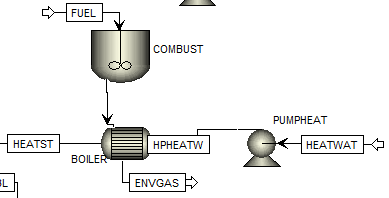
\includegraphics[width=.9\linewidth]{/home/vidianos/Documents/7o_εξάμηνο/Σχεδιασμός_Ι/Project/git_repo/Final_exam_files/Block_300_-_Λέβητας_Καύσης_Λιγνίνης/2023-01-10_18-51-18_screenshot.png}
\caption{Διάγραμμα Ροής του block 300}
\end{figure}

Στο block 300 παρουσιάζεται ο λέβητας της εγκατάστασης ο οποίος χρησιμοποιεί την λιγνίνη ως καύσιμο. Σκοπός του είναι η παραγωγή ατμού υψηλής πίεσης για χρήση ως θερμαντικό μέσο. Επίσης όμως, μπορεί να χρησιμοποιηθεί και για ηλεκτροπαραγωγή σε μία διάταξη όπως το κύκλο Rankine. Αυτό δεν υπάρχει ακόμη κάπου στην προσομοίωση, αλλά έχει θεωρηθεί πως όση από την ηλεκτρική ενέργεια μπορεί να παραχθεί από την λιγνίνη θα παραχθεί.

\subsection{Σχεδιαστικές Επιλογές}
\label{sec:org3cbc8ba}
Οι βασικές σχεδιαστικές επιλογές του λέβητα, είναι η πίεση στην οποία θα λειτουργεί ο λέβητας (πίεση εισόδου του νερού στον εναλλάκτη), ο βαθμός υπερθέρμανσης του λέβητα και οι συνθήκες λειτουργίας και ο τύπος του αντιδραστήρα.

Ο αντιδραστήρας που επιλέχθηκε είναι CSTR καθώς θέλουμε αντιδραστήρα συνεχούς ροής, για να υπάρχει συνεχή ροή καυσαερίων και άρα ατμοπαραγωγή που είναι το αποτέλεσμα του block αυτού. Ο CSTR αντιδραστήρας είναι η πιό απλή περίπτωση αντιδραστήρα συνεχούς ροής στην ανάλυση του και καθώς δεν είναι και από τους βασικούς αντιδραστήρες της διεργασίας, δεν έχουμε ασχοληθεί με πιθανά θέματα βελτιστοποίησης του. Ο αντιδραστήρας λειτουργεί σε πίεση 1 bar μη ισοθερμοκρασιακά. Η θερμογόνος δύναμη της λιγνίνης είναι γνωστή από βιβλιογραφία \textsuperscript{\citeprocitem{13}{13}} άρα μπορεί από αυτήν να υπολογιστεί η θερμοκρασία λειτουργίας του αντιδραστήρα η οποία είναι 1822 \(^oC\). Ο υπολογισμός έγινε στο χέρι και αποτελεί την αδιαβατική θερμοκρασία φλόγας και όχι την πραγματική. Όμως, ότι προσπάθεια έγινε να γίνει η προσομοίωση με δεδομένο heat duty και όχι θερμοκρασία έδινε errors, για αυτό ακολουθήθηκε αυτή η προσέγγιση. Επίσης πολύ σημαντικό σχεδιαστικό δεδομένο για έναν καυστήρα, είναι η περίσσεια άερα. Βρέθηκε σε βιβλιογραφία πως για την καύση πυρηνόξυλου, χρησιμοποιείται μία περίσσεια αέρα λ = 2.5. Παρόλο που η καύση γίνεται μόνο με την λιγνίνη και όχι όλο το πυρηνόξυλο, η τιμή του λ αυτή αναμένεται να είναι αρκετά κοντά άρα θεωρήθηκε μία περίσσεια αέρα της τάξης αυτής.

Ο λέβητας τώρα έχει ως σκοπό την παραγωγή ατμού υψηλής πίεσης, αφού τα καυσαέρια έχουν πολύ υψηλό θερμικό περιεχόμενο και μπορούν να παράξουν αυτόν τον ατμό. Η τιμή της πίεσης επιλέχθηκε στα 4 MPa η οποία είναι μία κλασσική πίεση λειτουργίας σε λέβητες υψηλής πίεσης. Η θερμοκρασία κορεσμού του ατμού στην πίεση αυτή είναι 250.4 \(^oC\). Ένας λέβητας παράγει τυπικά ελαφρώς υπέρθερμο ατμό, καθώς σε αρκετές περιπτώσεις (όπως στην ηλεκτροπαραγωγή), αυτός οδηγείται σε στρόβιλο στον οποίο πρέπει να μπαίνει υπέρθερμος ατμός και αν παραχθεί καθόλου μίγμα υγρού-ατμού αυτό να έχει υψηλή ποιότητα. Σε άλλη περίπτωση, θα υπάρξει μηχανολογικό πρόβλημα. Μέχρι τώρα, δεν υπάρχει κάτι τέτοιο στην διεργασία μας για να έχουμε μία καλή προσέγγιση του βαθμού υπερθέρμανσης που θέλουμε, για αυτό θεωρήθηκε ένας βαθμός υπερθέρμανσης του ατμού, λίγο πάνω από την θερμοκρασία κορεσμού του. Επιλέχθηκε αυθαίρετα η θερμοκρασία εξόδου 259 \(^oC\). 

\subsection{Υπολογισμοί}
\label{sec:org47e1b53}
Οι βασικοί υπολογισμοί της διεργασίας είναι η δυναμικότητα του λέβητα (πόσο ατμό υψηλής πίεσης παράγει ανά μονάδα χρόνου) και η κινητική του αντιδραστήρα.

Για την κινητική του αντιδραστήρα, θεωρήθηκε η εξής αντίδραση καύσης για την λιγνίνη
\[  C_{7.3}H_{13.9}O_{1.3} + 10.125O_2 \rightarrow 6.95 H_2O + 7.3CO_2  \] \textsuperscript{\citeprocitem{17}{17}} και βρέθηκε πως ακολουθεί κινητική πρώτης τάξης με ενέργεια ενεργοποίησης 46.68 kJ/mol και προεκθετικό παράγοντα 12.96 h\textsuperscript{-1} ή 3.6e-3 s\textsuperscript{-1} σε μονάδες SI \textsuperscript{\citeprocitem{18}{18}} . Βέβαια, αξίζει να αναφερθεί πως η μελέτη αυτή έγινε για lignin char και όχι για καθαρή λιγνίνη.

Για την δυναμικότητα του λέβητα, ξέρουμε ότι η τροφοδοσία έχει 5169 kg/hr λιγνίνη. Αν υποθέσουμε ότι όλη η λιγνίνη καίγεται σε έναν καυστήρα και τα καυσαέρια αυτού θερμαίνουν ατμό στα 4 MPa και 259 \(^oC\) σε έναν εναλλάκτη, προκύπτει πως μπορούμε να έχουμε ένα ρεύμα εξόδου 107.2 tn/h ατμό. Αξίζει να σημειωθεί πως δεν σταματάμε την εναλλαγή όταν το ΔΤ\textsubscript{min} των ρευμάτων γίνει πολύ μικρό, αλλά όταν η θερμοκρασία των καυσαερίων φτάσει κάτω από 150 \(^oC\). Γενικά σε χαμηλές θερμοκρασίες υπάρχει η ανησυχία συμπήκνωσης ισχυρών οξέων όπως το θειικό και το νιτρικό από τα οξείδια τους που μπορεί να υπάρχουν στον καυστήρα (παρότι στην περίπτωση μας έχουν αγνοηθεί). Επίσης, σε χαμηλές θερμοκρασίες, είναι δύσκολος ο ελκυσμός του λέβητα καθώς CO\textsubscript{2} το οποίο είναι βαρύτερο από τον αέρα μπορεί να τον φρακάρει. Στην προκειμένη έχει οριστεί θερμοκρασία εξόδου καυσαερίων 110 \(^oC\), αλλά εν γένει οι περισσότερες θερμοκρασίες πάνω από 100 \(^oC\) είναι καλές, καθώς το πυρηνόξυλο είναι υλικό μηδενικού θείου \textsuperscript{\citeprocitem{12}{12}}, άρα το θειικό οξύ το οποίο είναι ο βασικός μας φόβος που πηγαίνει την θερμοκρασία αυτή στους 150 \(^oC\) δεν μπορεί να σχηματιστεί.

Στην πράξη είναι μάλλον καλύτερο να εγκαθιστάται ένας μικρότερος λέβητας σε κάθε σημείο που υπάρχει η ανάγκη για να μην διακινείται ατμός υψηλής πίεσης για μεγάλες αποστάσεις. Καθώς ο βαθμός υπερθέρμανσης δεν είναι μεγάλος, σε μεγάλη απόσταση, μπορεί η πτώση πίεσης κατά μήκος του αγωγού να κάνει τον ατμό μίγμα υγρού-ατμού το οποίο θα μείωνε την αποδοτικότητα του. Αλλά, ο υπολογισμός αυτός είναι χρήσιμος για να ξέρουμε την μέγιστη δυνατή δυναμικότητα του εργοστασίου.

Το ιδανικό θα ήταν να μπορούσαμε να ξέρουμε πόση λιγνίνη απαιτείται για την παραγωγή μίας συγκεκριμένης ποσότητας ατμού, αλλά στην παρούσα φάση αυτό δεν έχει γίνει με μία μονοσήμαντη σχέση. Θεωρούμε πως ίσως να μπορεί να γίνει στο Aspen μέσω του Calculator, αλλά δεν έχει υπάρξει χρόνος για σχετικούς πειραματισμούς.

\subsection{Προσομοιώσεις στο Aspen}
\label{sec:org23f635c}
Το μοντέλο που χρησιμοποιήθηκε για την προσομοίωση είναι το SRK. Η καταστατική εξίσωση SRK είναι ιδανική για τον προσδιορισμό της μη ιδανικότητας της αέριας φάσης η οποία υπάρχει και είναι σε πολλά σημεία και σε υψηλή πίεση.

Στο Aspen τα δύο ρεύματα εισόδου είναι το νερό (του οποίου ποσότητα μεταβάλλουμε για να εκμεταλλευτούμε όσο το δυνατόν περισσότερη ενέργεια των καυσαερίων) και το καύσιμο μίγμα λιγνίνης και αέρα ο οποίος είναι σε περίσσεια 2.5 φορές από τον στοιχειομετρικό. Ο αντιδραστήρας της καύσης ορίστηκε σε πίεση 1 bar και θερμοκρασία 2095.6 Κ στον οποίο γίνεται αντίδραση καθαρά στην αέρια φάση εφόσον δεν υπάρχουν υγρά. Ο όγκος του αντιδραστήρα ορίστηκε ως 60 Mm\textsuperscript{3} το οποίο βρέθηκε πως είναι όγκος που πετυχαίνει πολύ υψηλή μετατροπή της λιγνίνης. Όπως αναφέρθηκε, δεν θα χρησιμοποιηθεί στην πράξη αυτός ο αντιδραστήρας αλλά θα σπάσει σε κομμάτια άρα αυτό δεν είναι και τόσο σημαντικό. Η κινητική του ορίστηκε ως ένα power law expression με την παραπάνω στοιχειομετρία, ειδική ταχύτητα και ενέργεια ενεργοποίησης.

Το νερό οδηγείται αρχικά σε αντλία με discharge pressure 4 MPa και έπειτα οδηγείται στον εναλλάκτη όπου εναλάσσει θερμότητα με τα καυσαέρια. Από το διάγραμμα T-q που δίνει το Aspen, μπορούμε να δούμε πόσο νερό μπορούμε να βάλουμε ώστε να εκμεταλλευτούμε όλη την θερμική ενέργεια των καυσαερίων μέχρι τους 100 \(^oC\) και λίγο παραπάνω σε κάθε περίπτωση.

\section{Ανάλυση του block 400 - Παραγωγή Γλυκερόλης}
\label{sec:org3208e0b}

\subsection{Διάγραμμα ροής και επεξήγηση}
\label{sec:org6addd15}
\begin{figure}[htbp]
\centering
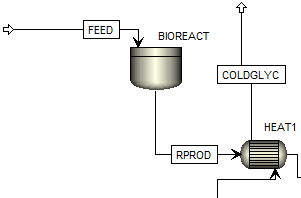
\includegraphics[width=.9\linewidth]{Διάγραμμα_ροής_και_Επεξήγηση/2023-01-12_16-53-41_screenshot.png}
\caption{Διάγραμμα ροής του block 400}
\end{figure}

Στο block 400 όπως προαναφέρθηκε γίνεται η παραγωγή της γλυκερόλης, ενός από τα δύο βασικά προιόντα στον βιοαντιδραστήρα, του οποίου το προιόν προθερμαίνεται με το ρεύμα της καθαρής γλυκερόλης του block 500. Στο διάγραμμα ροής φαίνονται ο βιοαντιδραστήρας και ο εναλλάκτης θερμότητας που απαιτούνται.

\subsection{Σχεδιαστικές Επιλογές}
\label{sec:orgbdcdfcf}
Η βασική σχεδιαστική επιλογή του block αυτού είναι ο τύπος και η λειτουργία του βιοαντιδραστήρα. Για τον εναλλάκτη δεν χρειάζεται να αναφερθεί κάτι καθώς ο σκοπός του είναι βασικά να ψύξει την παραγόμενη γλυκερόλη, το οποίο μπορεί να γίνει ταυτόχρονα με την προθέρμανση του ρεύματος εξόδου του αντιδραστήρα, άρα ήταν μία εύκολη επιλογή που βοηθάει στην ενεργειακή ολοκλήρωση της διεργασίας.

Για τον αντιδραστήρα, ο τύπος που επιλέχθηκε είναι ο αντιδραστήρας RBatch. Αυτό έγινε διότι η λειτουργία διαλείποντος έργου είναι αρκετά διαδεδομένη στους βιοαντιδραστήρες για 2 βασικούς λόγους. Ο πρώτος είναι πως οι αντιδράσεις αυτές έχουν αυτοκαταλυτική φύση άρα σε μία διάταξη συνεχούς ροής, υπάρχει βιομάζα στην έξοδο του αντιδραστήρα αντί να συσσωρεύεται όλη στον αντιδραστήρα, το οποίο μειώνει τον ρυθμό αντίδρασης, ενώ ο δεύτερος είναι ότι σε μία μικροβιακή καλλιέργεια, η οποία λειτουργεί σε μόνιμες συνθήκες, υπάρχει πάντα η πιθανότητα επιμόλυνσης του αντιδραστήρα. Στις περισσότερες περιπτώσεις, η επιμόλυνση αυτή δεν θα δράσει βοηθητικά για τον μικροοργανισμό μας και θα μειώσει τον ρυθμό της αντίδρασης και πιθανότατα την καθαρότητα του προιόντος. Όταν παρατηρηθεί κάτι τέτοιο, θα πρέπει να γίνει ολικό shut down του αντιδραστήρα και να καθαριστεί, το οποίο αποτελεί ένα μεγάλο διάστημα μη παραγωγικού χρόνου μέχρι να ξαναρχίσει το σύστημα σε μόνιμη κατάσταση. Στην περίπτωση του batch αντιδραστήρα, αυτός καθαρίζεται σε κάθε batch και λειτουργεί σε μη μόνιμη κατάσταση, άρα δεν χάνεται χρόνος για την αποκατάσταση της μόνιμης κατάστασης. Επίσης, είναι σημαντικά μικρότερη η πιθανότητα επιμόλυνσης.

Επιπλέον, ένας αντιδραστήρας CSTR πρέπει να λειτουργεί σε τέτοιες συνθήκες ώστε να μην οδηγηθεί σε μόνιμη κατάσταση έκπλυσης, κάτι το ανεπιθύμητο. Αυτό σημαίνει, πως για την τροφοδοσία του αντιδραστήρα μας, ο όγκος που απαιτείται είναι τουλάχιστον 3 φορές μεγαλύτερος αυτού του batch και αυτό είναι χωρίς να ληφθεί υπόψην η αργή κινητική, λόγω της οποίας ο όγκος μπορεί να είναι ακόμη μεγαλύτερος. Θεωρητικά, αυτό θα μπορούσε να λυθεί σε έναν αντιδραστήρα PFR, όμως η ανάδευση είναι ιδιαίτερα σημαντική στις αερόβιες μικροβιακές καλλιέργειες καθώς βοηθάει στην ομοιογένεια και στην συνεχή αιώρηση της βιομάζας, παράγοντες που επιτρέπουν την γρηγορότερη ανάπτυξη της. Επίσης, βελτιώνεται η διασπορά του δυσδιάλυτου οξυγόνου το οποίο πρέπει να υπάρχει και σε ορισμένες περιπτώσεις η μεταφορά του είναι από τα πιο βραδέα στάδια της διεργασίας. Για αυτό, οι αντιδραστήρες PFR δεν προτιμούνται συνήθως για τέτοιες διεργασίες, εκτός από ορισμένες περιπτώσεις κλινών στις οποίες υπάρχει ακινητοποιημένη βιομάζα, μία διεργασία η οποία είναι ιδιαίτερα περίπλοκη στην μελέτη της.

Όλοι αυτοί είναι λόγοι για τους οποίους δεν προτιμάται ένα σύστημα συνεχούς ροής, ακόμη και στην περίπτωση που θέλουμε πολύ υψηλή παραγωγικότητα στον αντιδραστήρα.

Για τις συνθήκες λειτουργίας του, εφόσον έχουμε μία καθαρή καλλιέργεια ενός μικροοργανισμού, οι βέλτιστες συνθήκες λειτουργίας είναι αυστηρά καθορισμένες από τον μικροοργανισμό και είναι τυπικά σε ένα στενό εύρος τιμών το οποίο βρίσκεται από βιβλιογραφία. Για τον μικροοργανισμό Candida glycerinogenes ο οποίος έχει χρησιμοποιηθεί στην διεργασία αυτή, βρέθηκε βιβλιογραφικά πως η βέλτιστη συγκέντρωση γλυκόζης είναι 230-250 g/l, η συγκέντρωση ουρίας 2 g/l, η συγκέντρωση φωσφόρου 55-60 mg/l (προστίθεται στην μορφή του corn steep liquor με βάση την βιβλιογραφία), το pH μεταξύ 4-6 και η θερμοκρασία μεταξύ 29 και 33 \(^oC\) \textsuperscript{\citeprocitem{10}{10}} . Για τα θρεπτικά συστατικά, βρέθηκε η ποσότητα νερού που απαιτείται για την παραγωγή διαλύματος γλυκόζης 230 g/l με όλη την γλυκόζη της διεργασίας και έπειτα η ποσότητα ουρίας και corn steep liquor (CSL) που απαιτείται ώστε οι συγκεντρώσεις τους να είναι οι επιθυμητές. Το pH δεν χρειάζεται να ρυθμιστεί σε κάποιο επίπεδο καθώς παρουσία του CSL το pH είναι στην επιθυμητή περιοχή ενώ η θερμοκρασία ρυθμίστηκε στους 30 \(^oC\) καθώς για αυτή την τιμή υπάρχουν κινητικά δεδομένα \textsuperscript{\citeprocitem{9}{9}} . Το CSL δεν προστέθηκε στην προσομοίωση της διεργασίας καθώς δεν υπάρχει στην βάση δεδομένων του Aspen και η πολυπλοκότητα της διεργασίας θα αυξανόταν σημαντικά με την προσθήκη του.

\subsection{Υπολογισμοί}
\label{sec:orgaf97123}
Οι βασικοί υπολογισμοί του block 400 είναι 3. Η στοιχειομετρία της μικροβιακής αντίδρασης, η οποία δεν είναι γνωστή εξ'αρχής, η κινητική της μικροβιακής αντίδρασης και οι υπολογισμοί του εναλλάκτη. Οι υπολογισμοί του εναλλάκτη έγιναν απευθείας στο Aspen για αυτό θα επεξηγηθούν περισσότερο στην προσομοίωση. Για την στοιχειομετρία και την κινητική της μικροβιακής αντίδρασης, βασιστήκαμε σε πειραματικά δεδομένα \textsuperscript{\citeprocitem{9}{9},\citeprocitem{10}{10}} . Ο προσδιορισμός της στοιχειομετρίας της αντίδρασης είναι μία περίπλοκη διαδικασία, ειδικά επειδή δεν είναι γνωστός εκ των προτέρων ο τύπος της βιομάζας. Υπάρχουν διάφορες τεχνικές που μπορούν να ακολουθηθούν για τον προσδιορισμό αυτόν, αλλά αποφασίστηκε πως αντί να υποτεθεί ο μοριακός τύπος της βιομάζας και να προκύψει μία αυθαίρετη μικροβιακή αντίδραση, να υπολογιστούν όσοι συντελεστές μπορούν με βάση τα πειραματικά δεδομένα για τα yields της αντίδρασης και να υπολογιστούν από αυτά ο τύπος της βιομάζας και όσοι στοιχειομετρικοί συντελεστές δεν είναι πειραματικά γνωστοί. Η αναλυτική επεξήγηση των υπολογισμών αυτών παρατίθεται στο παράρτημα Γ. Προκύπτει πως η αντίδραση είναι η

\[ 1.22 S + 0.24U + 2.89 O_2 \rightarrow 0.45 C_{1.48}H_{2.95}O_{0.048}N_{0.11} + G + 0.025E + 0.019Ac + 3.5CO_2 + 2.5H_2O \]
όπου S η γλυκόζη (υπόστρωμα), U η ουρία, G η γλυκερόλη, Ε η αιθανόλη και Ac το οξικό οξύ.

Για την κινητική της μικροβιακής αντίδρασης, έγινε προσαρμογή των παραπάνω πειραματικών δεδομένων στο μοντέλο Monod, το οποίο είναι το πιό κλασσικό μοντέλο για την μικροβιακή ανάπτυξη. Το πραγματικό κινητικό μοντέλο ενδέχεται να είναι πιό περίπλοκο από αυτό, αλλά απουσία μίας ολοκληρωμένης κινητικής μελέτης, το μοντέλο Monod είναι μία καλή πρώτη προσέγγιση. Ο ρυθμός με βάση το μοντέλο Monod είναι ο ρυθμός ανάπτυξης της βιομάζας. Με βάση την στοιχειομετρία όμως, ο ρυθμός της αντίδρασης ο οποίος θα χρησιμοποιηθεί στην διαστασιολόγηση του αντιδραστήρα θα είναι ο \(\frac{1}{0.45} \frac{dx}{dt}\).

Με βάση τα δεδομένα αυτά, το κινητικό μοντέλο που προέκυψε είναι το εξής:
\[ \frac{dx}{dt} = \frac{3.06*10^{-6}[S]}{236.19+[S]}[x] \] όπου οι σταθερές μ\textsubscript{max} και K\textsubscript{s} είναι υπολογισμένες σε μονάδες SI και οι συγκεντρώσεις σε g/l. Η προσαρμογή έγινε μέσω του Excel, το οποίο αρχείο μπορεί να βρεθεί \href{https://github.com/Vidianos-Giannitsis/Process-Design/blob/master/Calculations/c\_glycerinogenes\_kinetics.ods}{εδώ}.

\subsection{Προσομοιώσεις στο Aspen}
\label{sec:orgc1b71c5}
Το μοντέλο που χρησιμοποιήθηκε για την προσομοίωση είναι το NRTL-HOC. Το μοντέλο NRTL είναι ένα από τα πιο σύνηθη μοντέλα συντελεστών ενεργότητας, το οποίο είναι κατάλληλο για χημικά συστήματα σε χαμηλή πίεση. Η τροποποίηση των Hayden O' Connell στο μοντέλο αυτό χρησιμοποιείται όταν υπάρχουν μικρά οργανικά οξέα στο διάλυμα. Τα οξέα αυτά έχουν την ιδιαιτερότητα να μπορούν να αλληλεπιδράσουν μεταξύ τους με δεσμούς υδρογόνου στην αέρια φάση ακόμη και σε χαμηλές πιέσεις. Λόγω αυτών των αλληλεπιδράσεων, η αέρια φάση δεν μπορεί να θεωρηθεί ιδανική και για αυτό απαιτείται κάποια διόρθωση στο μοντέλο NRTL, την οποία πετυχαίνουν μοντέλα όπως το NRTL-HOC.

Το ρεύμα εισόδου της διεργασίας ορίστηκε με βάση τις συγκεντρώσεις που αναφέρθηκαν παραπάνω ως βέλτιστες. Έπειτα, ορίστηκε νερό ως ο διαλύτης σε μία ποσότητα τέτοια ώστε να υπάρχει όση γλυκόζη στο ρεύμα όση πρέπει να υπάρχει με βάση το block 200. Για τον βιοαντιδραστήρα, ορίστηκε ότι θα λειτουργεί σε σταθερή πίεση και θερμοκρασία (30 \(^oC\), 1 bar), με χρόνο λειτουργίας 80 ώρες (ο χρόνος που υπήρχε στα πειραματικά δεδομένα).

Το πιό ενδιαφέρον κομμάτι του βιοαντιδραστήρα είναι ότι μόλις βρούμε (με βάση την στοιχειομετρία και τα πειραματικά δεδομένα όπως περιγράφηκε παραπάνω) την βιομάζα του μικροοργανισμού, πρέπει αυτή να προσομοιωθεί στο Aspen. Η λογική που ακολουθήθηκε είναι η ίδια με αυτή που φαίνεται στο παράρτημα Β για την προσομοίωση της κυτταρίνης και της λιγνίνης ως conventional solids. Στην ίδια πηγή \textsuperscript{\citeprocitem{17}{17}} αναφέρεται και η προσομοίωση μίας βιομάζας, για αυτό με κάποιους υπολογισμούς, μπορούν εύκολα να υπολογιστούν τα χαρακτηριστικά της βιομάζας. Οι αναλυτικοί υπολογισμοί αυτοί φαίνονται στο παράρτημα Δ.

Για την κινητική, ορίστηκε η παραπάνω στοιχειομετρία, ενώ για την προσομοίωση του μοντέλου Monod, μπορεί να χρησιμοποιηθεί το μοντέλο LHHW με k=1, E=0, driving force τον αριθμητή του μοντέλου Monod και adsorption των παρανομαστή του. Αξίζει να αναφερθεί πως πρέπει οι μονάδες να είναι σε SI (όπως είναι στην προκειμένη περίπτωση) και στο Aspen πρέπει να μπούν οι λογάριθμοι των σταθερών και όχι οι ίδιες οι σταθερές. Επίσης, πρέπει να επιλεγεί το [C\textsubscript{i}] basis στο μενού του driving force ως mass concentration για να έχουν οι συγκεντρώσεις τις σωστές μονάδες.

Για τον εναλλάκτη του block, πρακτικά μας ενδιαφέρει να ψύξουμε το ρεύμα της καθαρής γλυκερόλης καθώς έτσι και αλλιώς δεν θα επαρκέσει για να φτάσει το ρεύμα την επιθυμητή θερμοκρασία. Για αυτό ψάχνουμε την χαμηλότερη θερμοκρασία που μπορούμε να πάμε το ρεύμα, η οποία προκύπτει πως είναι 44 \(^oC\), δηλαδή ένα ΔΤ = 14 \(^oC\) από την είσοδο του ψυχρού. Τα προιόντα του αντιδραστήρα είναι σε αρκετά μεγαλύτερη παροχή από ότι το ρεύμα αυτό, για αυτό στην αρχή του block 500 ολοκληρώνεται η θέρμανση αυτή.

\section{Ανάλυση του block 500 - Καθαρισμός Γλυκερόλης}
\label{sec:orgd80c6c3}

\subsection{Διάγραμμα ροής και Επεξήγηση}
\label{sec:org07e9853}
\begin{figure}[htbp]
\centering
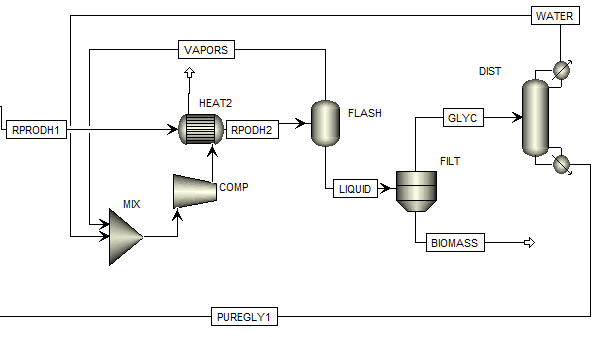
\includegraphics[width=.9\linewidth]{/home/vidianos/Documents/7o_εξάμηνο/Σχεδιασμός_Ι/Project/git_repo/Final_exam_files/Block_500_-_Καθαρισμός_Γλυκερόλης/2023-01-10_19-09-31_screenshot.png}
\caption{Διάγραμμα ροής του block 500}
\end{figure}

Στο block 500 γίνεται ο καθαρισμός του ρεύματος εξόδου του
βιοαντιδραστήρα παραγωγής γλυκερόλης. Αρχικά το ρεύμα προθερμαίνεται
και ύστερα εκτονώνεται σε έναν flash, στη συνέχεια εισέρχεται σε μία
φυγόκεντρο για την απομάκρυνση της στερέης φάσης, την βιομάζα, και τέλος
μια αποστακτική στήλη για τον τελικό καθαρισμό της γλυκερόλης.

\subsection{Σχεδιαστικές Επιλογές}
\label{sec:orgb580a96}
Το ρεύμα εξόδου προς καθαρισμό έχει 3 φάσεις, αέρια που είναι \(O_2\)
και \(CO_2\), στερεή που είναι βιομάζα, και υγρή που έχει νερό, οξικό
οξύ, γλυκερόλη, γλυκόζη, ουρία και αιθανόλη. Αρχικά επειδή το ρεύμα
έχει πολύ μεγάλη ποσότητα σε νερό, επιλέχθηκε ένας flash διαχωριστήρας,
εφόσον τα υγρά συστατικά έχουν χαμηλό σημείο βρασμού έως 120 \(^{o} C\)
πέρα από την γλυκερόλη που έχει σημείο βρασμού στους 290\(^{o} C\).
Παρακάτω παρουσιάζονται οι συνθήκες λειτουργίας στο flash.

\begin{table}[htbp]
\caption{Συνθήκες λειτουργίας του flash}
\centering
\begin{tabular}{ll}
Μέγεθος & Τιμή\\
\hline
Θερμοκρασία Εισόδου & 150 C\\
Θερμοκρασία Λειτουργίας & 140 C\\
Πίεση Λειτουργίας & 1 atm\\
\end{tabular}
\end{table}

Η πίεση παραμένει στη 1atm εφόσον δεν υπάρχει λόγος να αλλάξει εφόσον
υπάρχει μεγάλη διαφορά στα σημεία βρασμού μεταξύ του προιόντος και των
άλλων συστατικών. Η θερμοκρασία προθέρμανσης και λειτουργίας επιλέχθηκαν
έτσι ώστε να μην είναι αρκετά υψηλή για να υπάρξουν απώλειες σε
γλυκερόλη αλλά ούτε αρκετά χαμηλή που να παραμένει μεγάλη ποσότητα
νερού επειδή έτσι καθισταταί πιο ενεργοβόρα και κοστοβόρα η απόσταξη
αργότερα. Μετά απο διάφορες δοκιμές επιλέχθηκαν αυτές οι θερμοκρασίες
για τους παραπάνω λόγους.

Τέλος το ρεύμα καταλήγει σε μια αποστακτική στήλη για να απομακρυνθεί το
υπόλοιπο νερό ώστε να καθαριστεί πλήρως η γλυκερόλη, παράλληλα σε
αυτή την διεργασία απομακρύνεται όλη η εναπομένουσα αέρια φάση. Παρακάτω
παρουσιάζονται οι συνθήκες λειτουργίας στην αποστακτική στήλη τύπου
Radfrac.

\begin{table}[htbp]
\caption{Συνθήκες Λειτουργίας της Αποστακτικής}
\centering
\begin{tabular}{ll}
Μέγεθος & Τιμή\\
\hline
Θερμοκρασία εισόδου & 140 C\\
Θερμοκρασία λειτουργίας & 140 C\\
Πίεση κορυφής & 0.95 atm\\
Πίεση πυθμένα & 1.05 atm\\
Βαθμίδες & 6\\
Βαθμίδα Τροφοδοσίας & 3\\
Λόγος Αναρροής & 0.175\\
Λόγος αποστάγματος προς τροφοδοσία & 0.366\\
\end{tabular}
\end{table}

Η επιλογή των χαρακτηριστικών της στήλης έγιναν με βάση μια πρώτη
προσομοίωση με στήλη dstwu, ύστερα με βάση τα αποτελέσματά της έγινε
προσομοίωση σε radfrac. Η θερμοκρασία εισόδου και λειτουργίας δεν υπήρχε
λόγος να μεταβληθεί, όπως και η πίεση λειτουργίας λόγω της μεγάλης
διαφοράς στα σημεία βρασμού των υγρών συστατικών.

\subsubsection{Ενεργειακή Ολοκλήρωση}
\label{sec:org559fb75}
Η προθέρμανση του ρεύματος επιτυγχάνεται εξ ολοκλήρου από τα θερμά
ρεύματα της διεργασίας. Αρχικά το καθαρό ρεύμα γλυκερόλης, εξέρχεται
από την στήλη στους 290\(^{o} C\) , το οποίο είναι ακατάλληλο για
αποθήκευση σε κάποια δεξαμενή, για αυτόν τον λόγο χρησιμοποιείται για
προθέρμανση του ρεύματος για την είσοδο στο flash, όμως λόγο της χαμηλής
θερμοχωρητικότητας της σε σχέση με αυτή του νερού δεν μεταβάλλει την θερμοκρασία. Συνεπώς πρέπει
να αξιοποιηθούν τα αέρια ρεύματα του flash και της αποστακτικής στήλης.
Όμως επειδή αυτά βρίσκονται σε πίεση 1 atm όπως και το ψυχρό ρεύμα, δεν
επιτυγχάνεται επαρκή θέρμανση, για αυτό αν γίνει συμπίεση του θερμού
ρεύματος στις 2atm, ολοκληρώνεται η προθέρμανση του ρεύματος.

\subsection{Υπολογισμοί}
\label{sec:orgf3244d5}
Από τον βιοαντιδραστήρα παράγονται 13001 τόννοι γλυκερόλης τον
χρόνο, και από το τελικό ρεύμα ανακτούνται 11722 τόνοι, που αποτελεί το
90\%, δηλαδή χάνεται το 10\% της παραγόμενης γλυκερόλης στα αέρια
ρεύματα του flash και της αποστακτικής. Επίσης το τελικό ρεύμα
γλυκερόλης έχει καθαρότητα 99,99\%.

\subsection{Προσομοιώσεις στο Aspen}
\label{sec:org40cfaa6}
Το μοντέλο που χρησιμοποιήθηκε για την προσομοίωση είναι το NRTL-HOC. Εφόσον το ρεύμα αυτό είναι συνέχεια του block 400, έχει τα ίδια συστατικά και άρα η αιτιολόγηση του μοντέλου είναι η ίδια. Το ρεύμα εισόδου της διεργασίας είναι στην ουσία τα προιόντα της βιοαντίδρασης όπως βγαίνουν από το block 400. Οδηγείται στους εναλλάκτες, οι οποίοι χρησιμοποιήθηκαν για την θέρμανση του και έπειτα μπαίνει στο flash.

Για τον διαχωρισμό της βιομάζας χρησιμοποιήθηκε ένα CFuge με το μοντέλο Decanter η οποία είναι η βασική διεργασία του Aspen για τον διαχωρισμό υγρού στερεού. Αυτό τοποθετήθηκε μετά το flash για να επιβεβαιωθεί ότι το μίγμα που τροφοδοτείται σε αυτόν δεν έχει αέρια φάση, όπως θα συνέβαινε αν ο decanter αυτός ήταν στην έξοδο του βιοαντιδραστήρα επειδή δεν υπάρχει πρότυπη μέθοδος για διαχωρισμό στερεού από μίγμα υγρού-ατμού.

Για την αποστακτική στήλη, αρχικά αυτή προσομοιώθηκε ως DSTWU ορίζοντας ελαφρύ (νερό) και βαρύ κλειδί (γλυκερόλη), ένα reflux ratio το οποίο δεν είναι ανάγκη να είναι σωστό σε πρώτη φάση, πτώση πίεσης στην στήλη και ορίζοντας την ανάκτηση στο απόσταγμα ώστε να έχει αρκετά μικρή ποσότητα γλυκερόλης (για να μην υπάρχουν απώλειες) και σχεδόν όλο το νερό. Από τα αποτελέσματα της στήλης αυτής βρέθηκαν οι σχεδιαστικές παραμέτροι που απαιτεί η στήλη Radfrac και προσομοιώθηκε με αυτά.

\section{Block 600 - Παραγωγή Κυκλοπεντανόνης με την Φουρφουράλη ως ενδιάμεσο προϊόν}
\label{sec:orgaf411ea}

\subsection{Διάγραμμα ροής και Επεξήγηση}
\label{sec:orga385d8a}
\begin{figure}[htbp]
\centering
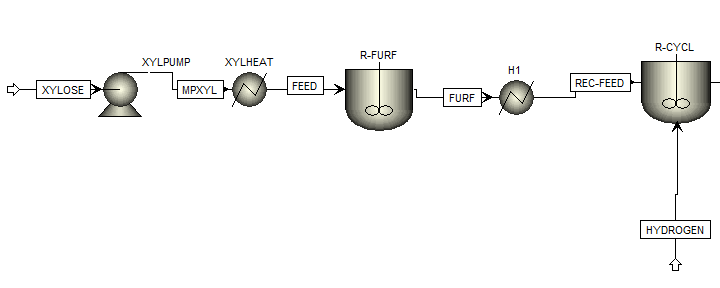
\includegraphics[width=.9\linewidth]{Block_600_-_Παραγωγή_Κυκλοπεντανόνης_με_την_Φουρφουράλη_ως_ενδιάμεσο_προϊόν/2023-01-13_17-51-52_screenshot.png}
\caption{Διάγραμμα ροής του block 600}
\end{figure}

Η κυκλοπεντανόνη παράγεται από τη προσθήκη υδρογόνου στο ενδιάμεσο
προϊόν της διαδικασίας που ονομάζεται φουρφουράλη, η οποία προέρχεται
από την αφυδάτωση στης ξυλόζης. Για αυτό το στάδιο, λοιπόν, από το steam
explosion αξιοποιείται το ρεύμα της ημικυτταρινικής φάσης της βιομάζας
που περιέχει ως κύριο συστατικό την ξυλόζη και εισέρχεται στο block
διεργασίας 600. Στη παρούσα εργασία έχει γίνει η παραδοχή ότι η
ημικυτταρινική φάση αποτελείται από καθαρό ρεύμα ξυλόζης, βέβαια στην
πραγματικότητα το ρεύμα έχει και άλλα συστατικά τα οποία πρέπει να
ληφθούν υπόψιν. Οι εναλλάκτες και η αντλία της διάταξης είναι για να λειτουργεί το σύστημα στις σωστές συνθήκες πίεσης και θερμοκρασίας κάθε αντιδραστήρα.

\subsection{Παραγωγή φουρφουράλης}
\label{sec:orgbe8a621}
\subsubsection{Σχεδιαστικές Επιλογές}
\label{sec:org0b9f750}
Για το block 600 οι δύο βασικές σχεδιαστικές επιλογές είναι ο τύπος και
η λειτουργία των αντιδραστήρων R-FURF και R-CYCL. Όπως φαίνεται από το
διάγρμμα ροής, το ρεύμα ξυλόζης αρχικά συμπιέζεται από την αντλία
XYLPUMP και προθερμένεται από τον θερμαντήρα XYLHEAT πριν εισέρθει σε
ένα αντιδραστήρα συνεχούς έργου R-FURF.

Ο τύπος αντιδραστήρα που επιλέκτηκε είναι CSTR. Οι αντιδραστήρες CSTR
χρησιμοποιούνται συχνά από τη βιβλιογραφία \textsuperscript{\citeprocitem{19}{19}} για
αυτή την αντίδραση, λόγω της απλότητας στον σχεδιασμό και την λειτουργία
τους. Πιο αναλυτικά, επιλέχτηκε αντιδραστήρας συνεχής ροής διότι για να
διασπαστεί μεγάλη ποσότητα ξυλόζης σε φουρφουράλη και νερό είναι
απαραίτητο ο αντιδραστήρας να βρίσκεται σε μόνιμες συνθήκες με υψηλή
θερμοκρασία, περίπου 200 με 250 \(^oC\). Σε αυτή τη θερμοκρασία η ξυλόζη
βρίσκεται σε υγρή φάση, ενώ η φουρφουράλη και το νερό σε αέρια. Τα κύρια
οφέλη των αντιδραστήρων συνεχής ροής είναι ότι ο χρόνος παραμονής έιναι
μικρός και το προϊόν αφαιρείται αμέσως από την υγρή φάση, άρα
αποφεύγονται αντιδράσεις απώλειας φουφουράλης που μπορεί να συμβούν στην
υγρή φάση και να μειώσουν την απόδοση της διεργασίας. Θα μπορούσε να
χρησιμοποιηθεί αντιδραστήρας PFR, όπως συμβαίνει αρκετά συχνά στην
βιβλιογραφία \textsuperscript{\citeprocitem{20}{20}–\citeprocitem{22}{22}}, όμως η απόδοση
της διεργασίας θα ήταν χαμηλότερη, διότι δεν θα υπήρχε καλός έλεγχος της
θερμοκρασίας κατά μήκος του αντιδραστήρα. Αντίθετα, η συνεχής ανάδευση
της ξυλόζης που λαμβάνει χώρα στον αντιδραστήρα CSTR είναι απαραίτητη
γιατι συμβάλλει στην μεταφορά θερμότητας και μάζας.

Η χρήση ενός batch αντιδραστήρα θα είχε χαμηλή αποδοτικότητα αφού λόγω
του μεγαλύτερου χρόνου παραμονής θα μπορούσαν να υπάρχουν απώλειες
φουρφουράλης στην υγρή φάση και δεν θα υπήρχε καλή μεταφοράς μάζας \textsuperscript{\citeprocitem{19}{19}}. Συνεπώς η διαδικασία θα είχε πολύ χαμηλές
αποδόσεις και θα σπαταλούσε σημαντικά ποσά ενέργειας. Τέλος, η
τροφοδοσία ξυλόζης είναι πολύ μεγάλη και προτιμάται συνεχής ροή για
διεργασίες μεγάλου μεγέθους.

Συνεπώς, επιλέκτηκε το μοντέλο CSTR διότι δίνει υψηλότερη μετατροπή και
επιλεκτικότητα σε φουρφουράλη σε σχέση με αντιδραστήρες PFR και Batch
και υπάρχουν επαρκή δεδομένα κινητικής στην βιβλιογραφία \textsuperscript{\citeprocitem{19}{19}} .

Ο αντιδραστήρας, σύμφωνα με την βιβλιογραφία \textsuperscript{\citeprocitem{19}{19}} ,
λειτουργεί σε σταθερή πίεση 15.6 atm και θερμοκρασία 242\textsuperscript{o}C ώστε το
ρεύμα εξόδου να έχει την επιθυμητή σύσταση.

\subsubsection{Υπολογισμοί}
\label{sec:org9f11e1a}
Στις συνθήκες που προαναφέρθηκαν, υπολογίστηκε ότι η ξυλόζη διασπάται σε
νερό και φουρφουράλη με την εξής στοιχειομετρία:

C\textsubscript{5}H\textsubscript{10}O\textsubscript{5} → 3H\textsubscript{2}O + C\textsubscript{5}H\textsubscript{4}O\textsubscript{2}

\subsubsection{Προσομοιώσεις στο Aspen}
\label{sec:org5d0f375}
Στην είσοδο του αντιδραστήρα ως τροφοδοσία θεωρείται το ημικυτταρινικό
κλάσμα με κύριο συστατικό την ξυλόζη με μαζική παροχή 3808,7 kg/h, όπως
υπολογίστηκε από το steam explosion, ενώ η έξοδος του αντιδραστήρα είναι
πλούσια σε φουρφουράλη και νερό. Οι συνθήκες λειτουργίας του
αντιδραστήρα ορίστηκαν ως σταθερή πίεση 15.6 atm και θερμοκρασία
242\textsuperscript{o}C.

Για τις θερμοδυναμικές παραμέτρους χρησιμοποιήθηκε το θερμοδυναμικό
μοντέλο PRWS που βασίζεται στην καταστατική εξίσωση
Peng-Robinson-Wong-Sandler. Το μοντέλο αυτό μπορεί να χρησιμοποιηθεί σε
πολικά και μη πολικά συστατικά, για υψηλές θερμοκρασίες και πιέσεις
μέχρι 150 bar.

Η αντίδραση περιγράφεται από τον μηχανισμό Powerlaw και από την
βιβλιογραφία \textsuperscript{\citeprocitem{19}{19}} ο προεκθετικός παράγοντας Α της αντίδρασης ισούται με
7,92*10\textsuperscript{20} και η ενέργεια ενεργοποίησης είναι 167,9 kJ/mol.

Το ρεύμα που εξέρχεται από τον αντιδραστήρα R-FURF είναι πλούσιο σε
φουρφουράλη και νερό. Η φουρφουράλη είναι απαραίτητη για την παραγωγή
της κυκλοπεντανόνης και πρέπει να σταλεί στο επόμενο στάδιο. Το ρεύμα
αυτό οδηγείται σε έναν εναλλάκτη θερμότητας Η1 έτσι ώστε να ψυχθεί. Για
την προσομοίωση της ψύξης του μίγματος χρησιμοποιήθηκε το μοντέλο
Heater. Ορίστηκε θερμοκρασία 160\textsuperscript{o}C και πίεση 15,8 bar, για να
προσαρμόσει τις συνθήκες του ρεύματος φουρφουράλης πριν εισαχθεί στον
επόμενο αντιδραστήρα, χρησιμοποιώντας επίσης το θερμοδυναμικό μοντέλο
PRWS.

\subsection{Παραγωγή Κυκλοπεντανόνης}
\label{sec:orgda9d537}
\subsubsection{Σχεδιαστικές επιλογές}
\label{sec:org9e18fac}
Σε αυτό το στάδιο σχεδιασμού για τον αντιδραστήρα R-CYCL επιλέχτηκε o
αντιδραστήρας CSTR. Αυτό συνέβη διότι ο αντιδραστήρας λειτουργεί σε
συνθήκες εξόδου οπότε η πίεση παραμένει σταθερή σε όλα τα στάδια.
Επιπλέον, το ρεύμα τροφοδοσίας που εισέρχεται στον αντιδραστήρα είναι
μεγάλου μεγέθους (3.968 kg/hr) οπότε προτιμάται αντιδραστήρας συνεχής
ροής αφού μπορεί να ελέγχεται καλύτερα ο χρόνος παραμονής, η θερμοκρασία
και η πίεση ώστε το προϊόν να έχει σταθερή ποιότητα, σε σχέση με batch
αντιδραστήρες. Ακόμη, εάν ο αντιδραστήρας ήταν batch, ο χρόνος
λειτουργίας θα ήταν μικρότερος από τον χρόνο που δεν θα λειτουργούσε,
οπότε δεν θα συνέφερε πρακτικά και οικονομικά στην διεργασία.

\subsubsection{Υπολογισμοί:}
\label{sec:orgf3687be}
Η στοιχειομετρία της αντίδρασης υπολογίστηκε ως εξής:

C\textsubscript{5}H\textsubscript{4}O\textsubscript{2} + 3H\textsubscript{2} → H\textsubscript{2}O + C\textsubscript{5}H\textsubscript{8}O

\subsubsection{Προσομοιώσεις στο Aspen}
\label{sec:org2fe79c3}
Το ρεύμα φουρφουράλης και νερού, με την ίδια σύσταση που είχαν στην
έξοδο του αντιδραστήρα R-FURF, εισέρχονται στον R-CYCL. Ταυτόχρονα,
εισέρχεται ποσότητα υδρογόνου, τέτοια ώστε η καθαρότητα της κυκλοπεντανόνης
να είναι \(98 \%\).

Οι συνθήκες λειτουργίας του αντιδραστήρα καθορίστηκαν σε σταθερή
θερμοκρασία 160\textsuperscript{ο}C και πίεση 4 MPa. Για τη μοντελοποίηση του
αντιδραστήρα, ορίστηκε η κινητική της αντίδρασης με το μηχανισμό
Powerlaw, που από την βιβλιογραφία \textsuperscript{\citeprocitem{1}{1}} η σταθερά της
αντίδρασης για 160\textsuperscript{ο}C είναι ίση με 0,0128 hr\textsuperscript{-1} με ενέργεια
ενεργοποίησης 64,2 kJ/mol. Ο χρόνος που χρειάζεται η αντίδραση για να
πραγματοποιηθεί σε αυτές τις συνθήκες είναι 1 ώρα. Το θερμοδυναμικό
μοντέλο που επιλέχθηκε είναι το PRWS, λόγω της υψηλής θερμοκρασίας.

Αυτό έχει ως αποτέλεσμα η έξοδος του αντιδραστήρα να έχει μαζική παροχή
3968,2 kg/hr όπου η κυκλοπεντανόνη αποτελεί το 2103,5 kg/hr. Τα υπόλοιπα
προιόντα και η σύσταση αυτών παρουσιάζονται στον πίνακα 1 του
παραρτήματος Ε.

Το ρεύμα που εξέρχεται από τον αντιδραστήρα R-CYCL δεν είναι καθαρή
κυκλοπεντανόνη οπότε κατευθύνεται στο επόμενο τμήμα, το Block 700. Εκεί
πραγματοποιείται η αφαίρεση και ανακύκλωση του εναπομείναντος υδρογόνου,
το οποίο βρίσκεται στην αέρια φάση και ο καθαρισμός της κυκλοπεντανόνης.

\section{Block 700 - Καθαρισμός της Κυκλοπεντανόνης}
\label{sec:org5e03e00}
\subsection{Διάγραμμα ροής και Επεξήγηση}
\label{sec:org0e8727a}
\begin{figure}[htbp]
\centering
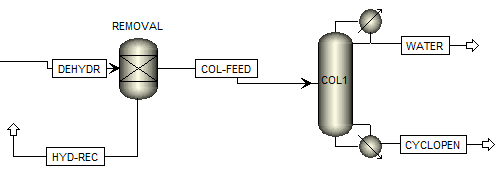
\includegraphics[width=.9\linewidth]{Block_700_-_Καθαρισμός_της_Κυκλοπεντανόνης/2023-01-13_18-02-03_screenshot.png}
\caption{Διάγραμμα ροής του block 700}
\end{figure}

Στο Block 700 λαμβάνει χώρα ο καθαρισμός κυκλόπεντανόνης. Αρχικά, το
ρεύμα εξόδου από τον αντιδραστήρα R-CYCL κατευθύνεται προς έναν
διαχωριστήρα, με σκοπό την αφαίρεση και ανακύκλωση εναπομείναντος
υδρογόνου, το οποίο βρίσκεται στην αέρια φάση. Στη συνέχεια, το ρεύμα
που είναι πλούσιο σε κυκλοπεντανόνη διοχετεύεται σε μια αποστακτική
στήλη, όπου συμβαίνει ο διαχωρισμός για την παραλαβή καθαρής
κυκλοπεντανόνης.

\subsection{Σχεδιαστικές Επιλογές}
\label{sec:org1de117a}
Οι δύο βασικές σχεδιαστικές επιλογές του block 700 είναι ο τύπος και η
λειτουργία των δύο στηλών διαχωρισμού.

Για τον διαχωρισμό υδρογόνου χρησιμοποιήθηκε το Component Separator
διότι ο σκοπός είναι να διαχωριστεί το υδρογόνο από το μίγμα
κυκλοπεντανόνης και να χρησιμοποιηθεί με ανακύκλωση στον αντιδραστήρα
R-CYCL. Στην πράξη, καθώς το υδρογόνο είναι ένα αέριο με πολύ χαμηλότερο σημείο βρασμού από ότι όλα τα υπόλοιπα συστατικά, μάλλον μπορεί να ανακτηθεί όλη η ποσότητα του υδρογόνου με ένα flash. Όμως, δεν υπήρχε χρόνος για να δοκιμαστεί αυτό στο Aspen.

Για τον καθαρισμό της κυκλοπεντανόνης χρησιμοποιήθηκε αποστακτική στήλη
DSTWU. Αυτή η αποστακτική στήλη είναι απλή και λειτουργεί με ένα ρεύμα
τροφοδοσίας και δύο προϊόντα απόσταξης. Θα μπορούσε να χρησιμοποιηθεί
κάποια άλλη στήλη όπως η Distl ή η RadFrac, αλλά αυτές πραγματοποιούν
πιο περίπλοκους υπολογισμούς και χρειάζονται περισσότερα δεδομένα.
Επιπλέον, δεν υπάρχει αζεότροπο στο ρεύμα, οπότε δεν χρειάζεται μία πιό αναλυτική επίλυση της στήλης με ένα μοντέλο όπως η στήλη RadFrac.

\subsection{Προσομοιώσεις στο Aspen και Υπολογισμοί:}
\label{sec:org2d07629}
Στο Aspen χρησιμοποιήθηκε Component Separator με το θερμοδυναμικό
μοντέλο Peng Robinson με κανόνες ανάμιξης Wong-Sandler (PRWS) για την
πρόβλεψη των θερμοδυναμικών ιδιοτήτων του συστήματος. Για αυτόν λοιπόν
τον separator η πίεση είναι στα 40 bar, ίδιο με την πίεση εξόδου από τον
αντιδραστήρα κυκλοπεντανόνης, και το μίγμα μέσα σε αυτόν είναι διφασικό
(υγρό-ατμός). Μέσω την χρήση του διαχωριστή, το μίγμα που προκύπτει από
τον αντιδραστήρα διαχωρίζεται σε δύο ρεύματα: Το ένα ρεύμα περιέχει
εξολοκλήρου υδρογόνο, το οποίο ανακυκλώνεται στον αντιδραστήρα της
κυκλοπεντανόνης, ενώ το άλλο ρεύμα που περιέχει την κυκλοπεντανόνη, την
φουρφουράλη και το νερό προχωράει στην αποστακτική στήλη για περεταίρω
επεξεργασία.

Πριν να φτάσει το ρεύμα στην αποστακτική στήλη ψύχεται σε εναλλάκτη
θερμότητας σε θερμοκρασία 160 \^{}\{ο\}C και πίεση 20 bar. Το θερμοδυναμικό
μοντέλο για τον εναλλάκτη είναι το ίδιο (PRWS). Στο Aspen ως
εναλλάκτης θερμότητας εφαρμόστηκε Heater. Μετά τη ψύξη του, το ρεύμα
εισέρχεται σε μια αποστακτική στήλη με σκοπό τον διαχωρισμό της
κυκλοπεντανόνης από το νερό.

Αρχικά έγινε χρήση του Azeotrope Finder για την εύρεση αζεότροπων, αλλά
διαπιστώθηκε πως σε πίεση 16 bar δεν υπάρχουν αζεότροπα. Εφόσον η πίεση
του μίγματος είναι 40 bar από τον αντιδραστήρα υδρογόνωσης, επιλέχθηκε
να γίνει απόσταξη σε πίεση 16 bar. Λόγω της έλλειψης αζεότροπων, στο
Aspen έγινε χρήση της απλοποιημένης στήλης DSTWU. Η στήλη περιέχει 55
βαθμίδες απόσταξης και ως προϊόν κορυφής ανακτάται το νερό κατά \(99.9 \%\).
Στο προϊόν κορυφής επιλέγεται η κυκλοπεντανόνη να ανακτάται σε ποσοστό
\(7.7 \%\), εφόσον μικρότερα ποσοστά οδηγούν σε υπερβολικά μεγάλο αριθμό
βαθμίδων και λόγων αναρροής. Η πίεση στον συμπυκνωτή όσο και στον
αναβραστήρα είναι 16 bar, δηλαδή θεωρείται πως δεν υφίσταται πτώση
πίεσης μέσα στην στήλη. Από τους υπολογισμούς του Aspen προκύπτουν τα αποτελέσματα του παρακάτω πίνακα

\begin{table}[htbp]
\caption{Χαρακτηριστικά της αποστακτικής στήλης}
\centering
\begin{tabular}{lr}
Μέγεθος & Τιμή\\
\hline
Ελάχιστος Λόγος Αναρροής & 0.96\\
Πραγματικός Λόγος Αναρροής & 6.61\\
Ελάχιστος Αριθμός Βαθμίδων & 49.39\\
Πραγματικός Αριθμός Βαθμίδων & 55\\
Λόγος αποστάγματος προς τροφοδοσία & 0.813\\
Βαθμίδα τροφοδοσίας & 32\\
\end{tabular}
\end{table}

Ως αποτέλεσμα, το ρεύμα κορυφής έχει μαζική παροχή 1971,2 kg/hr με το
νερό να αποτελεί το \(92.3 \%\) της συνολικής μάζας, και το ρεύμα πυθμένα έχει
μαζική παροχή 1988,7 kg/hr και η κυκλοπεντανόνη αποτελεί το \(98.2 \%\) της
συνολικής μάζας. Τα αποτελέσματα της αποστακτικής στήλης βρίσκονται στον
πίνακα 2. του παραρτήματος.

Στον πίνακα 3. του παραρτήματος απεικονίζονται συνολικά οι μαζικές
παροχές αλλά και οι συστάσεις όλων των ρευμάτων που λαμβάνου χώρα τόσο
για τη παραγωγή όσο και τον καθαρισμό της κυκλοπεντανόνης.

\section{Συμπεράσματα και Προτάσεις για την Διεργασία}
\label{sec:org024b2ba}
\subsection{Συμπεράσματα}
\label{sec:orgc1f518c}
Συνοπτικά, μια βασική διαδικασία για την παραγωγή κυκλοπεντανόνης και γλυκερόλης από πυρηνόξυλο έχει σχεδιαστεί, κοστολογηθεί και αναλυθεί με χρήση διάφορων διεργασιων. Η διαδικασία αποδείχθηκε ότι έχει θετικό οικονομικό δυναμικό, με μικρό κόστος πρώτων υλών και είναι φιλική προς το περιβάλλον. Καθώς τα προιόντα αυτά έχουν ζήτηση, ιδιαίτερα για φαρμακοβιομηχανίες, θεωρούμε πως αξίζει να γίνει μία επένδυση στην διεργασία αυτή. Βέβαια, η διεργασία απαιτεί πολύ περισσότερη μελέτη για να είναι ολοκληρωμένη η εικόνα μας για αυτήν.

\subsection{Προτάσεις}
\label{sec:orgc0f7e79}
Το βασικότερο που πρέπει να γίνει είναι μία ολοκληρωμένη οικονομική ανάλυση της διεργασίας, όπου θα κοστολογηθεί ο εξοπλισμός, οι βοηθητικές παροχές και η ηλεκτρική ενέργεια που απαιτείται για την διεργασία έτσι ώστε να αξιολογηθεί καλύτερα η επένδυση.
\subsubsection{Βελτιώσεις στις προσομοιώσεις}
\label{sec:org2fe986e}
Αρχικά, ορισμένες από τις προσομοιώσεις έχουν παραδοχές για την απλοποίηση των προσομοιώσεων οι οποίες στην τελική μελέτη πιθανόν να μπορούν να αρθούν. Έχουν ήδη αναφερθεί παραπάνω μερικές μικρές παραβλέψεις που έχουν γίνει σε ορισμένες προσομοιώσεις, αλλά μία βασική βελτίωση είναι πως πρέπει στην προσομοίωση της κυκλοπεντανόνης (block 600) να οριστεί το πραγματικό ρεύμα ξυλόζης, το οποίο έχει ορισμένες ακαθαρσίες οι οποίες θα δυσχεραίνουν τους διαχωρισμούς της διεργασίας. Επίσης οι εναλλάκτες αυτού του block πρέπει να προσομοιωθούν με χρήση βοηθητικών παροχών και όχι μόνο με το απλό μοντέλο heater.

\subsubsection{Βελτιώσεις στην διεργασία}
\label{sec:org8e91853}
Επίσης όμως, θα γίνουν και κάποιες βελτιώσεις στην διεργασία. Η βασικότερη θα είναι να γίνει μία ολοκληρωμένη ενεργειακή ολοκλήρωση της διεργασίας και να εκμεταλλευτούν όλα τα ψυχρά και θερμά ρεύματα που έχουμε διαθέσιμα. Επίσης σημαντικό όταν αρχίσουμε να λαμβάνουμε υπόψην τις βοηθητικές παροχές και την ηλεκτρική ενέργεια είναι ότι το block 300 που περιέχει την καύση της λιγνίνης είναι ακόμη σε πρώιμο στάδιο και δείχνει μόνο πως θα παραχθεί ατμός στον λέβητα. Στην πράξη, αυτός ο ατμός μπορεί να χρησιμοποιηθεί σε ένα κύκλο Rankine για παράδειγμα για ηλεκτροπαραγωγή και ταυτόχρονα να μπεί στην διεργασία και μία μονάδα τηλεθέρμανσης για την καλύτερη εκμετάλλευση του. Καθώς η ποσότητα λιγνίνης που ανακτάται είναι αρκετά μεγάλη, η δυναμικότητα του λέβητα είναι υψηλή και μπορεί να καταφέρει να καλύψει μεγάλο ποσό των ενεργειακών και θερμικών αναγκών της εγκατάστασης.

Επίσης, η κυκλοπεντανόνη που παράγεται έχει καθαρότητα 0.98, το οποίο πρέπει να βελτιωθεί, καθώς η κυκλοπεντανόνη που χρησιμοποιείται συνήθως έχει καθαρότητα 0.99. Μία άλλη ενδιαφέρουσα βελτίωση της διεργασίας είναι πως ο μικροοργανισμός που χρησιμοποιείται στην παραγωγή της γλυκερόλης έχει δύο σημαντικά παραπροιόντα, την αιθανόλη και το οξικό οξύ, τα οποία παράγονται σε ποσότητες της τάξης των 140 tn/y. Παρότι μικρές ποσότητες για την κλίμακα της εγκατάστασης, θα μπορούσαν να διαχωριστούν αυτά από το νερό και να πωληθούν, το οποίο είναι ένα σενάριο που μπορεί να εξεταστεί περαιτέρω.

\pagebreak

\section{Βιβλιογραφία}
\label{sec:org704b232}
\hypertarget{citeproc_bib_item_1}{(1) Yu, Z.; Li, Y.; Yao, Y.; Wang, Y.; Liu, Y.-Y.; Sun, Z.; Shi, C.; Wang, W.; Wang, A. Highly Selective Hydrogenative Ring-Rearrangement of Furfural to Cyclopentanone over a Bifunctional Ni3P/\$\gamma\$-Al2O3 Catalyst. \textit{Molecular catalysis} \textbf{2022}, \textit{522}, 112239. \url{https://doi.org/10.1016/j.mcat.2022.112239}.}

\hypertarget{citeproc_bib_item_2}{(2) Shen, T.; Hu, R.; Zhu, C.; Li, M.; Zhuang, W.; Tang, C.; Ying, H. Production of Cyclopentanone from Furfural over Ru/C with Al11.6PO23.7 and Application in the Synthesis of Diesel Range Alkanes. \textit{Rsc advances} \textbf{2018}, \textit{8} (66), 37993–38001. \url{https://doi.org/10.1039/C8RA08757A}.}

\hypertarget{citeproc_bib_item_3}{(3) Werpy, T.; Petersen, G. Top Value Added Chemicals from Biomass: Volume I – Results of Screening for Potential Candidates from Sugars and Synthesis Gas. \textbf{2004}, DOE/GO-102004–101992, 15008859. \url{https://doi.org/10.2172/15008859}.}

\hypertarget{citeproc_bib_item_4}{(4) Leiva-Candia, D. E.; Pinzi, S.; Redel-Macías, M. D.; Koutinas, A.; Webb, C.; Dorado, M. P. The Potential for Agro-Industrial Waste Utilization Using Oleaginous Yeast for the Production of Biodiesel. \textit{Fuel} \textbf{2014}, \textit{123}, 33–42. \url{https://doi.org/10.1016/j.fuel.2014.01.054}.}

\hypertarget{citeproc_bib_item_5}{(5) Patel, A.; Arora, N.; Sartaj, K.; Pruthi, V.; Pruthi, P. A. Sustainable Biodiesel Production from Oleaginous Yeasts Utilizing Hydrolysates of Various Non-Edible Lignocellulosic Biomasses. \textit{Renewable and sustainable energy reviews} \textbf{2016}, \textit{62}, 836–855. \url{https://doi.org/10.1016/j.rser.2016.05.014}.}

\hypertarget{citeproc_bib_item_6}{(6) Chintagunta, A.; Zuccaro, G.; Kumar, M.; Kumar, S.; Garlapati, V.; Postemsky, P.; Kumar, N.; Chandel, A.; Simal-Gandara, J. Biodiesel Production From Lignocellulosic Biomass Using Oleaginous Microbes: Prospects for Integrated Biofuel Production. \textit{Frontiers in microbiology} \textbf{2021}, \textit{12}. \url{https://doi.org/10.3389/fmicb.2021.658284}.}

\hypertarget{citeproc_bib_item_7}{(7) Semkiv, M. V.; Ruchala, J.; Dmytruk, K. V.; Sibirny, A. A. 100 Years Later, What Is New in Glycerol Bioproduction? \textit{Trends in biotechnology} \textbf{2020}, \textit{38} (8), 907–916. \url{https://doi.org/10.1016/j.tibtech.2020.02.001}.}

\hypertarget{citeproc_bib_item_8}{(8) Wang, Z.; Zhuge, J.; Fang, H.; Prior, B. A. Glycerol Production by Microbial Fermentation: A Review. \textit{Biotechnology advances} \textbf{2001}, \textit{19} (3), 201–223. \url{https://doi.org/10.1016/S0734-9750(01)00060-X}.}

\hypertarget{citeproc_bib_item_9}{(9) Jin, H.; Fang, H.; Zhuge, J. By-Product Formation by a Novel Glycerol-Producing Yeast, Candida Glycerinogenes, with Different O2 Supplies. \textit{Biotechnology letters} \textbf{2003}, \textit{25} (4), 311–314. \url{https://doi.org/10.1023/A:1022349401575}.}

\hypertarget{citeproc_bib_item_10}{(10) Zhuge, J.; Fang, H.-Y.; Wang, Z.-X.; Chen, D.-Z.; Jin, H.-R.; Gu, H.-L. Glycerol Production by a Novel Osmotolerant Yeast Candida Glycerinogenes. \textit{Applied microbiology and biotechnology} \textbf{2001}, \textit{55} (6), 686–692. \url{https://doi.org/10.1007/s002530100596}.}

\hypertarget{citeproc_bib_item_11}{(11) Domalski, E. S.; Jobe, T. L.; Milne, T. A. Thermodynamic Data for Biomass Conversion and Waste Incineration - NREL. \textbf{1987}, 326.}

\hypertarget{citeproc_bib_item_12}{(12) Gonzalez, J. F.; Gonzalez-Garcia, C. M.; Ramiro, A.; Gonzalez, J.; Sabio, E.; Ganan, J.; Rodrıguez, M. A. Combustion Optimisation of Biomass Residue Pellets for Domestic Heating with a Mural Boiler. \textit{Biomass and bioenergy} \textbf{2004}, \textit{27} (2), 145–154. \url{https://doi.org/10.1016/j.biombioe.2004.01.004}.}

\hypertarget{citeproc_bib_item_13}{(13) Fernandez-Bolanos, J.; Felizon, B.; Heredia, A.; Guillen, R.; Jimenez, A. Characterization of the Lignin Obtained by Alkaline Delignification and of the Cellulose Residue from Steam-Exploded Olive Stones. \textit{Bioresource technology} \textbf{1999}, \textit{68} (2), 121–132. \url{https://doi.org/10.1016/S0960-8524(98)00134-5}.}

\hypertarget{citeproc_bib_item_14}{(14) Koutsomitopoulou, A. F.; Bénézet, J. C.; Bergeret, A.; Papanicolaou, G. C. Preparation and Characterization of Olive Pit Powder as a Filler to PLA-matrix Bio-Composites. \textit{Powder technology} \textbf{2014}, \textit{255}, 10–16. \url{https://doi.org/10.1016/j.powtec.2013.10.047}.}

\hypertarget{citeproc_bib_item_15}{(15) Fernandez-Bolanos, J.; Felizon, B.; Heredia, A.; Rodriguez, R.; Guillen, R.; Jimenez, A. Steam-Explosion of Olive Stones: Hemicellulose Solubilization and Enhancement of Enzymatic Hydrolysis of Cellulose. \textit{Bioresource technology} \textbf{2001}, \textit{79} (1), 53–61. \url{https://doi.org/10.1016/S0960-8524(01)00015-3}.}

\hypertarget{citeproc_bib_item_16}{(16) Roy, A. K.; Bag, S. C.; Sardar, D.; Sen, S. K. Infrared Spectra of Jute Stick Bleached with Sodium Chlorite and Hydrogen Peroxide. \textit{Journal of applied polymer science} \textbf{1991}, \textit{43} (12), 2187–2192. \url{https://doi.org/10.1002/app.1991.070431205}.}

\hypertarget{citeproc_bib_item_17}{(17) Wooley, R. J.; Putsche, V. Development of an ASPEN PLUS Physical Property Database for Biofuels Components. \textbf{1996}, 36.}

\hypertarget{citeproc_bib_item_18}{(18) Farrokh, N. T.; Suopajärvi, H.; Sulasalmi, P.; Fabritius, T. A Thermogravimetric Analysis of Lignin Char Combustion. \textit{Energy procedia} \textbf{2019}, \textit{158}, 1241–1248. \url{https://doi.org/10.1016/j.egypro.2019.01.413}.}

\hypertarget{citeproc_bib_item_19}{(19) Nhien, L. C.; Long, N. V. D.; Lee, M. Novel Hybrid Reactive Distillation with Extraction and Distillation Processes for Furfural Production from an Actual Xylose Solution. \textit{Energies} \textbf{2021}, \textit{14} (4), 1152. \url{https://doi.org/10.3390/en14041152}.}

\hypertarget{citeproc_bib_item_20}{(20) Ershova, O.; Kanervo, J.; Hellsten, S.; Sixta, H. The Role of Xylulose as an Intermediate in Xylose Conversion to Furfural: Insights via Experiments and Kinetic Modelling. \textit{Rsc advances} \textbf{2015}, \textit{5} (82), 66727–66737. \url{https://doi.org/10.1039/C5RA10855A}.}

\hypertarget{citeproc_bib_item_21}{(21) Papaioannou, M.; Kleijwegt, R. J. T.; van der Schaaf, J.; Neira d’Angelo, M. F. Furfural Production by Continuous Reactive Extraction in a Millireactor under the Taylor Flow Regime. \textit{Industrial \& engineering chemistry research} \textbf{2019}, \textit{58} (35), 16106–16115. \url{https://doi.org/10.1021/acs.iecr.9b00604}.}

\hypertarget{citeproc_bib_item_22}{(22) Carrasco, F. Production of Furfural by Dilute-Acid Hydrolysis of Wood: Methods For Calculating Furfural Yield. \textit{Wood and fiber science} \textbf{1993}, 91–102.}

\hypertarget{citeproc_bib_item_23}{(23) Liggett, R. W.; Koffler, H. CORN STEEP LIQUOR IN MICROBIOLOGY. \textit{12}, 15.}

\pagebreak

\section{Παράρτημα Α - Ισοζύγια Μάζας για την έκρηξη ατμού}
\label{sec:org1161d51}
Μελετάμε τα yields της έκρηξης ατμού με βάση τους \textsuperscript{\citeprocitem{15}{15}} .

Βλέπουμε πως πιό αποδοτική είναι η διεργασία για Τ = 232 C και χρόνο παραμονής 2 λεπτά, με Ro = 4.22. Σε αυτήν, η υδατοδιαλυτή φάση είναι το 25.5\% του συνολικού ενώ στην στερεή φάση ανακτάται το 52.9\% της βιομάζας εκ του οποίου το 37.7\% είναι στο κλάσμα της κυτταρίνης και το 15.2\% της λιγνίνης.

Στην υγρή φάση είναι η ημικυτταρίνη και φαινόλες. Αφαιρόντας την σύσταση των φαινολών (2.5\%) βρίσκουμε πως ανακτήθηκε το 93.8\% της συνολικής ημικυτταρίνης. Το υπόλοιπο ή διασπάστηκε θερμικά κατά την διεργασία ή δεν διαλύθηκε. Ακόμη, από την σύσταση της φάσης αυτής, ξέρουμε ότι το 51.4\% είναι ζάχαρες, δηλαδή έχουμε ως προιόν 26214 tn ημικυτταρινικές ζάχαρες. Οι φαινόλες θεωρούμε πως ανακτόνται πλήρως μέσω εκχύλισης, ενώ τα υπόλοιπα πηγαίνουν στον αντιδραστήρα παραγωγής φουρφουράλης όπου δραστική είναι μόνο η ξυλόζη ενώ τα υπόλοιπα συστατικά θα υποθέσουμε ότι είναι αδρανή. Η ξυλόζη είναι το 45.7\% της υδατοδιαλυτής φάσης, άρα η τροφοδοσία της θα είναι 23307 tn/y.

Από τη στερεή φάση, βλέπουμε πόση λιγνίνη ανακτάται το οποίο είναι το 62.8\% της συνολικής. Στην κυτταρινική φάση υπάρχει περίσεμα ποσότητας καθώς βγαίνει μεγαλύτερη από την κυτταρίνη που υπάρχει στο δείγμα. Τα υπόλοιπα είναι λιγνίνη που δεν αφαιρέθηκε και αδιάλυτη ημικυτταρίνη.

Για να δούμε πόση κυτταρίνη έχει πραγματικά το κλάσμα αυτό, πρέπει να σκεφτούμε τι διασπάστηκε. Για αυτό, δεν υπάρχουν λεπτομερή δεδομένα και απαιτείται να γίνουν κάποιες παραδοχές, αλλά ξέρουμε πως η ημικυτταρίνη είναι η πιό επιρρεπής στην θερμική διάσπαση και άρα μπορούμε να υποθέσουμε πως ότι δεν διαλύθηκε διασπάστηκε θερμικά ενώ η λιγνίνη είναι η πιό θερμοάντοχη. Άρα, πέρα από την ημικυτταρίνη, ένα σημαντικό ποσοστό της θερμικά αποδομημένης βιομάζας θα είναι κυτταρίνη. Επίσης, πέρα από τις φαινόλες της λιγνίνης, μπορούμε να υποθέσουμε πως δεν διαλύθηκε άλλη ποσότητα κυτταρίνης ή λιγνίνης στο νερό άρα ότι απώλεια έχουμε είναι θερμική. Η απώλεια λιγνίνης είναι 37.2\%. Θα υποθέσουμε ότι μόνο ένα 10\% αυτού είναι θερμική διάσπαση καθώς η θερμοκρασία είναι σχετικά χαμηλή για την λιγνίνη. Άρα διασπάστηκε ένα 3.72\% της συνολικής λιγνίνης.

Υπό αυτές τις παραδοχές, βρίσκουμε ότι το κυτταρινικό κλάσμα έχει 60486 tn κυτταρίνη και 14914 tn λιγνίνη. Άρα, ανακτάται το 81.74\% της συνολικής κυτταρίνης, και το κλάσμα αυτό είναι κατά 19.78\% λιγνίνη. Έπειτα, το κλάσμα αυτό ακολουθεί κατεργασία με ClO\textsubscript{2} το οποίο σε όξινες συνθήκες οξειδώνει την λιγνίνη και δημιουργεί ίζημα το οποίο διαχωρίζεται με διήθηση. Το ρεύμα της καθαρής πλέον κυτταρίνης (60486 tn/y) υδρολύεται 

Έπειτα, η κυτταρίνη αυτή υδρολύεται παράγοντας γλυκόζη με την μέγιστη δυνατή απόδοση (εφόσον έχει απολιγνοποιηθεί). Αυτό είναι 30.9\% της μάζας του ξηρού υποστρώματος της έκρηξης ατμού, δηλαδή των 105800 tn/y. Άρα, παράγονται 32692.2 tn/y γλυκόζη. Αυτή είναι η γλυκόζη που μπαίνει στον βιοαντιδραστήρα ως υπόστρωμα.

\section{Παράρτημα Β - Ορισμός Κυτταρίνης και Λιγνίνης ως Conventional Solids}
\label{sec:orgb83a185}
Σύμφωνα με τους \textsuperscript{\citeprocitem{17}{17}}, η κυτταρίνη αντιστοιχεί σε ένα πολυμερές με δομική μονάδα το μόριο \(C_6H_{10}O_5\) για αυτό θα χρησιμοποιηθεί η ένωση αυτή στην προσομοίωση. Για την λιγνίνη υποτέθηκε ο τύπος \(C_{7.3}H_{13.9}O_{1.3}\). Οι αντίστοιχες αντιδράσεις καύσης είναι οι
\begin{align*}
C_6H_{10}O_5 + 6O_2 \rightarrow 5H_2O + 6CO_2 \\ C_{7.3}H_{13.9}O_{1.3} + 10.125O_2 \rightarrow 6.95 H_2O + 7.3CO_2
\end{align*} 

Με βάση αυτούς, απαιτείται μοριακό βάρος, θερμότητα και ενέργεια gibbs της σύνθεσης, θερμοχωρητικότητα και ειδικός όγκος για να οριστεί ένα conventional solid.

Για την κυτταρίνη, το μοριακό βάρος υπολογίζεται άμεσα για τη δομική μονάδα (162.144). Η θερμότητα σύνθεσης βρέθηκε βιβλιογραφικά \textsuperscript{\citeprocitem{11}{11}} ως 17.456 MJ/kg το οποίο αντιστοιχεί σε 2.83e+6 kJ/kmol ενώ η ενέργεια Gibbs βρέθηκε από την αντίστοιχη ενέργεια Gibbs της καύσης ως 4.783 kJ/kmol. Για την θερμοχωρηστικότητα, βρέθηκε από τους \textsuperscript{\citeprocitem{17}{17}} ότι για Τ = 298.15 Κ, CP\textsubscript{s} = 0.117e+5 και για Τ = 1000 K, CP\textsubscript{s} = 0.672e+3. Η πυκνότητα θεωρήθηκε 1.5 g/cc (ίδια με του αμύλου). Άρα, 0.667 cc/g αν θέλουμε ειδικό όγκο ή 108.15 cc/mol αν θέλουμε γραμμομοριακό όγκο.

Για την λιγνίνη, το μοριακό βάρος υπολογίζεται και εδώ άμεσα (122.493). Η θερμότητα σύνθεσης βρέθηκε συγκεκριμένα για πυρηνόξυλο ως 23.5 MJ/kg (2.879e+6 kJ/kmol) από τους \textsuperscript{\citeprocitem{13}{13}}, η γραμμομοριακή ενέργεια Gibbs 6.1762 kJ/kmol μέσω την ενέργειας Gibbs της καύσης ενώ η θερμοχωρητικότητα από την βάση δεδομένων του NREL ως \(0.25660 + 3.22 \cdot 10^{-3} T\) (J/g K) ή \(31.43 + 0.3944 T\) (J/mol K). H πυκνότητα υποτέθηκε και εδώ ίση με του αμύλου αλλά καθώς το Aspen θέλει γραμμομοριακό όγκο, αυτός υπολογίστηκε ως 81.7 cc/mol.

\section{Παράρτημα Γ - Στοιχειομετρία Βιοαντιδραστήρα}
\label{sec:orgd92d9e4}

Η βιοαντίδραση που θα χρησιμοποιηθεί είναι μία περίπλοκη αντίδραση της οποίας η στοιχειομετρία μπορεί πολύ δύσκολα να προσδιοριστεί ακριβώς. Επειδή απαιτείται μία έκφραση χημικής αντίδρασης για να μπεί στο ασπεν, θα γίνει μία προσέγγιση της παραγωγής προιόντων με βάση τις ποσότητες που παράγονται. Η αντίδραση που θα υποτεθεί είναι η
\[ S + U + C \rightarrow G + Ar + E + Ac\]
όπου S = γλυκόζη (substrate), U = ουρία, C = CSL, G = γλυκερόλη, Ar = αραβιτόλη, Ε = αιθανόλη, Ac = οξικό οξύ
δηλαδή πως η γλυκόζη "διασπάται" σε γλυκερόλη, αιθανόλη, οξικό οξύ και αραβιτόλη.

Στην πράξη η αντίδραση αυτή είναι αερόβια (πρέπει να υπάρχει οξυγόνο στα αντιδρώντα), αφορά την ανάπτυξη ενός μικροοργανισμού (πρέπει να υπάρχει βιομάζα στα προιόντα) και θα έχει και νερό και CO\textsubscript{2} ως προιόντα όπως όλες οι μικροβιακές αντιδράσεις. Λόγω έλλειψης δεδομένων, στο ασπεν, η αντίδραση θα μοντελοποιηθεί με βάση το παραπάνω.

Στην αντίδραση συμμετέχουν 32692.2 tn γλυκόζη, 283.74 tn ουρία και 567.57 tn CSL. Όμως, βάση προηγούμενων παραδοχών, έχουμε πει πως δεν αντιδρά όλη η ουρία και όλο το CSL. Έχουμε υποθέσει ότι αντιδρούν τα 3/4 της ουρίας και το μισό CSL. Άρα, 212.8 tn ουρία και 283.79 tn CSL. Τα προιόντα είναι 13643 tn γλυκερόλη, 640.68 tn αραβιτόλη, 168.82 tn αιθανόλη και 165.99 tn οξικό οξύ. Αρχικά, πρέπει να μετατρεπούν οι ποσότητες αυτές σε mol και έπειτα, από τις αναλογίες τους να βρεθούν οι συντελεστές. Ως βάση των υπολογισμών θα χρησιμοποιηθεί το 1 mol γλυκερόλης.

Οι \href{https://github.com/Vidianos-Giannitsis/Process-Design/blob/master/Calculations/bioreactor\_stoichiometry.m}{σχετικοί υπολογισμοί} φαίνονται στο ομώνυμο αρχείο matlab στον φάκελο /Calculations.

Η στοιχειομετρία της αντίδρασης που προκύπτει είναι
\[ 1.22S + 0.024U + 0.049C \rightarrow G + 0.028Ar + 0.025E + 0.019Ac \]
Αξίζει να αναφερθεί πως το CSL ορίστηκε ως ένα συστατικό με την σύσταση που φαίνεται στον παρακάτω πίνακα από την οποία προκύπτει ο εμπειρικός τύπος
\(C_{0.94}H_{2.94}O_{1.41}N_{0.04}P_{0.03}K_{0.03}\)
\begin{table}[htbp]
\caption{Σύσταση του CSL στα συστατικά του}
\centering
\begin{tabular}{lr}
Συστατικό & Περιεκτικότητα\\
\hline
Νερό & 0.6\\
Γαλακτικό Οξύ & 0.15\\
Ζάχαρες σε ισοδύναμη & 0.05\\
συγκέντρωση γλυκόζης & \\
Τέφρα & 0.1\\
Αμινοξέα σε ισοδύναμη & 0.03\\
συγκέντρωση αλανίνης & \\
Αμμωνία & 0.01\\
Φώσφορος & 0.03\\
Κάλιο & 0.03\\
\hline
Άθροισμα & 1\\
\end{tabular}
\end{table}

Αξίζει να αναφερθεί πως στον πίνακα αυτό έχουν υπερεκτιμηθεί ορισμένα από τα συστατικά σε σχέση με τις τιμές τους στην αντίστοιχη βιβλιογραφία \textsuperscript{\citeprocitem{23}{23}}. Αυτό συμβαίνει επειδή με βάση τις τιμές εκείνες ήταν αδύνατον να αθροιστούν τα συστατικά στη μονάδα.

Εφόσον στην αντίδραση αυτή δεν έχουν συμπεριληφθεί O\textsubscript{2} στα αντιδρώντα και βιομάζα, H\textsubscript{2O} και CO\textsubscript{2} στα προιόντα, δεν θα κλείνουν τα στοιχειακά ισοζύγια για την αντίδραση. Απουσία άλλων δεδομένων, οι συντελεστές Ο\textsubscript{2}, CO\textsubscript{2}, H\textsubscript{2O} και βιομάζας θα ληφθούν όλοι ίσοι με την μονάδα και ο τύπος της βιομάζας θα προκύψει έτσι ώστε να κλείνει το ισοζύγιο. Αν συμπεριληφθούν O\textsubscript{2} στα αντιδρώντα και CO\textsubscript{2}, H\textsubscript{2O} στα προιόντα όλα με συντελεστή μονάδα, τότε προκύπτει πως η βιομάζα θα έχει τύπο \(C_{3.167}H_{4.333}O_{3.217}N_{0.05}\). Άρα, η συνολική μικροβιακή αντίδραση που διεξάγεται θα είναι η
\[ 1.22S + 0.24U + 0.049C + O_2 \rightarrow C_{3.167}H_{4.333}O_{3.217}N_{0.05} + G + 0.028Ar +0.025E + 0.019Ac + H_2O +CO_2 \]

Σε πρώτη φάση, μπορεί η προσωμοίωση να γίνει στην απλουστευμένη περίπτωση ότι γλυκόζη και οξυγόνο, δίνουν γλυκερόλη, διοξείδιο του άνθρακα και νερό, κυρίως για να εξοικειωθώ με τους batch αντιδραστήρες στο ασπεν και να δοκιμάσω κάτι. Σε επόμενη φάση θα αναλυθεί η παραπάνω συνολική αντίδραση και οι διαχωρισμοί που απαιτεί. Για την στοιχειομετρία της αντίδρασης \(C_6H_{12}O_6 + O_2 \rightarrow C_3H_8O_3 + CO_2 +H_2O\) έχουμε 2 βαθμούς ελευθερίας ενώ οι υπόλοιποι συντελεστές καθορίζονται από τα mass balances C, H, O. Αν υποθέσουμε ότι οι συντελεστές γλυκερόλης και γλυκόζης είναι ίδιοι με αυτούς της συνολικής αντίδρασης τότε έχουμε ένα πλήρως ορισμένο σύστημα. Και καθώς αυτά τα δύο προκύπτουν από τα ίδια πειραματικά δεδομένα με την κινητική, είναι μία έγκυρη πηγή. Άρα, σε πρώτη φάση θα εξεταστεί η αντίδραση
\(1.22 C_6H_{12}O_6 + 3.82O_2 \rightarrow C_3H_8O_3 + 4.32CO_2 + 3.32H_2O\) .

Όπως έχει αναφερθεί στα αρχεία των σχετικών προσομοιώσεων, ο ρυθμός της αντίδρασης αυτής είναι πολύ μεγαλύτερος από ότι θα έπρεπε με αποτέλεσμα η αντίδραση να τελειώνει σε μισή ώρα. Μάλλον, αυτό που φταίει είναι ότι παράγεται πολύ βιομάζα. Όμως, διαπιστώθηκε πως ο συντελεστής της βιομάζας δεν είναι πραγματικά μονάδα, αλλά ξέρουμε την τελική συγκέντρωση της βιομάζας στον αντιδραστήρα. Όμως, δεν μπορούμε να ξέρουμε τον ακριβή στοιχειομετρικό συντελεστή αν δεν ξέρουμε τον μοριακό τύπο, για αυτό η γνώση αυτή προσθέτει μία παραπάνω εξίσωση. Ακόμη, ξέρουμε πως ο αντιδραστήρας λειτουργεί τυπικά με αερισμό 0.1-0.5 vvm (volume of air per volume of liquid per minute). Άρα, είναι γνωστός ο συντελεστής του οξυγόνου και δεν αποτελεί άγνωστο. Άρα, οι εξισώσεις που διαμορφώνονται είναι 5 με 7 αγνώστους.

Το σύστημα είναι ως εξής
\begin{align*}
4.167 = SbCb + S_{CO2} \\ 6.333 = SbHb + 2S_{H_2O} \\ 4.94 = SbOb + 2S_{CO2} + S_{H_2O} \\ 0.05 = SbNb \\ Sb = \frac{10.385}{12Cb+16Ob+Hb+14Nb}
\end{align*} 

Η επίλυση του συστήματος αυτού είναι αρκετά δύσκολη και έγινε με την fsolve του Matlab. Λόγω της πολυπλοκότητας του συστήματος, απαιτείται αρκετό trial and error για να βρεθεί το σύστημα σε μία ευσταθή λύση και ακόμη περισσότερο για να βρεθεί λύση που έχει νόημα (όλοι οι άγνωστοι είναι θετικοί και ο στοιχειομετρικός συντελεστής βιομάζας είναι μικρότερος του 1). Στο trial and error αυτό, μεταβαλλόντουσαν όχι μόνο οι αρχικές συνθήκες του αλγορίθμου αλλά και οι βαθμοί ελευθερίας του συστήματος. Καθώς οι συντελεστές CO\textsubscript{2} και H\textsubscript{2}O προκαλούν του ίδιου τύπου μεταβολές στο σύστημα και η αύξηση τους οδηγεί απομάκρυνση από το σημείο ισορροπίας μετά από ένα σημείο, θεωρήθηκε απαραίτητο να μεταβληθεί και η παροχή οξυγόνου και να μην χρησιμοποιηθεί η βιβλιογραφική.

Το σύστημα μπόρεσε να συγκλίνει για τις εξής τιμές των 8 αγνώστων:
\begin{center}
\begin{tabular}{lr}
Άγνωστος & Τιμή\\
\hline
S\textsubscript{b} & 0.4519\\
C\textsubscript{b} & 1.48\\
H\textsubscript{b} & 2.95\\
O\textsubscript{b} & 0.048\\
N\textsubscript{b} & 0.11\\
S\textsubscript{O2} & 2.89\\
S\textsubscript{CO2} & 3.5\\
S\textsubscript{H2O} & 2.5\\
\end{tabular}
\end{center}
και αρχικές τιμές S\textsubscript{b} = 5, C\textsubscript{b} = 0.208, H\textsubscript{b} = 0.3165, O\textsubscript{b} = 0.247, N\textsubscript{b} = 2.5e-4. Είναι σίγουρο πως το σύστημα έχει πολλές λύσεις και αυτή δεν είναι η μοναδική που βγάζει νόημα, αλλά εφόσον βρέθηκα κάποια που βγάζει και λόγω της πολυπλοκότητας που εμπεριέχεται στο να βρεί κανείς μία λογική λύση για το σύστημα αυτό, η προσομοίωση θα προχωρήσει με αυτό.

Για το σύστημα αυτό όμως δεν ισχύει το συνολικό ισοζύγιο μάζας, παρόλο που ικανοποιούνται όλα τα μερικά. Το συνολικό ισοζύγιο μάζας ικανοποιείται αν και μόνο αν \[ 117.38 + 32S_O = 44S_{CO2} + 18S_{H_2O} \]. Η ποσότητα βιομάζας είναι γνωστή και είναι 10.385. Αλλά ανάλογα με το Sb που βγαίνει, πρέπει να επιβεβαιώσουμε ότι το σύστημα έχει δώσει το κατάλληλο μοριακό βάρος για να είναι το γινόμενο τους 10.385. Διατηρώντας σταθερά τα S\textsubscript{CO}\textsubscript{2} και S\textsubscript{H2O} που χρησιμοποιήθηκαν παραπάνω, βρέθηκε πως πρέπει το S\textsubscript{O2} να είναι 2.55. Δίνοντας τους βαθμούς ελευθερίας αυτούς στο παραπάνω σύστημα και επιλύοντας το με αρχική τιμή τη προηγούμενη λύση, ο αλγόριθμος κάνει exit με τον κωδικό 3, που σημαίνει ότι δεν κατάφερε να συγκλίνει σε λύση επειδή η επαναληπτική διαδικασία ξεπέρασε το tolerance της. Όμως, το σφάλμα στην επίλυση είναι αρκετά μικρό. Αν αλλάξουμε τον άνθρακα της λύσης που δίνει έτσι ώστε το μοριακό βάρος να βγαίνει τέτοιο ώστε να ισχύει το συνολικό ισοζύγιο μάζας, τότε μάλλον είμαστε καλά. Δοκιμάζοντας αυτό παίρνουμε τον παρακάτω πίνακα για τις μεταβλητές του συστήματος.
\begin{center}
\begin{tabular}{lr}
Άγνωστος & Τιμή\\
\hline
S\textsubscript{b} & 0.1087\\
C\textsubscript{b} & 6.225\\
H\textsubscript{b} & 12.369\\
O\textsubscript{b} & 0.1133\\
N\textsubscript{b} & 0.4736\\
S\textsubscript{O2} & 2.55\\
S\textsubscript{CO2} & 3.5\\
S\textsubscript{H2O} & 2.5\\
\end{tabular}
\end{center}

Περνόντας τα καινούργια αυτά δεδομένα στο ασπεν και επιβεβαιώνοντας ότι η παροχή οξυγόνου στην τροφοδοσία επαρκεί για την αντίδραση (και δεν είναι σε μεγάλη περίσσεια επειδή δεν υπάρχει λόγος), το ασπεν τρέχει κανονικά την προσομοίωση και βγάζει τα σωστά αποτελέσματα για την ροή μάζας της βιομάζας του μικροοργανισμού στην έξοδο του αντιδραστήρα. Αξίζει να σημειωθεί πως για να είναι σωστός ο ρυθμός της αντίδρασης, πρέπει να διαιρέσουμε την σταθερά στο driving force με τον στοιχειομετρικό συντελεστή της βιομάζας καθώς ο ρυθμός που έχει εισαχθεί είναι ο ρυθμός παραγωγής βιομάζας (μοντέλο Monod). Ο χρόνος παραμονής που προκύπτει δεν έχει καμία απολύτως σχέση και πάλι, αλλά πλέον η προσομοίωση είναι σίγουρα (περίπου, κανείς δεν είναι βέβαιος ποιά είναι η πραγματική λύση του συστήματος) σωστή. 

\section{Παράρτημα Δ - Προσομοίωση της βιομάζας στο Aspen}
\label{sec:org5be1ab3}
Για την ολοκληρωμένη προσωμοίωση της βιοαντίδρασης, απαιτείται μοντελοποίηση της βιομάζας του μικροοργανισμού C. glycerinogenes στο Aspen. Αυτό είναι δύσκολο διότι δεν υπάρχουν πολλές πληροφορίες για αυτό. Όμως, σύμφωνα με τους \textsuperscript{\citeprocitem{17}{17}} ο μοριακός τύπος της βιομάζας (ο οποίος μπορεί να προκύψει μέσω της στοιχειομετρίας της) αρκεί για όλα τα δεδομένα που θεωρεί απαραίτητα το Aspen. Η βιομάζα μπορεί να οριστεί ως ένα conventional solid στο Aspen. Για αυτό, τα δεδομένα που χρειάζεται το Aspen είναι τα εξής: Μοριακό βάρος, θερμότητα σύνθεσης, θερμοχωρητικότητα και πυκνότητα.

Ο μοριακός τύπος υπολογίζεται με τη βοήθεια του αρχείου biomass\textsubscript{properties} ο οποίος χρησιμοποιεί τους υπολογισμούς της στοιχειομετρίας για να προσδιορίσει τον τύπο της βιομάζας. Ο τύπος που προκύπτει είναι ο \(C_{3.33}H_{4.72}O_{3.38}N_{0.05}P_{0.0015}\) . Το μοριακό βάρος υπολογίζεται απευθείας από τα ατομικά βάρη C, H, O, N, P ως MW = 99.592 g/mol. Η πυκνότητα του υλικού μπορεί να υποτεθεί παρόμοια του αμύλου (περίπου 1.5 g/ml). Για την θερμοχωρητικότητα του υλικού, μπορεί να χρησιμοποιηθεί \href{https://en.wikipedia.org/wiki/Kopp\%27s\_law}{ο κανόνας του Kopp} ο οποίος λέει ότι η θερμοχωρητικότητα ενός υλικού μπορεί να προσδιοριστεί από τα στοιχεία του ως \[ C = \sum_{i=1}^{N} C_{i}f_i \] σε \(\left[ \frac{J}{kg \cdot K} \right]\) όπου C\textsubscript{i} η θερμοχωρητικότητα του κάθε στοιχείου στις μονάδες αυτές και f\textsubscript{i} το κλάσμα μάζας του στοιχείου. Ο νόμος αυτός δουλεύει καλά σε χαμηλές θερμοκρασίες, στις οποίες γίνεται και η βιοαντίδραση. Για την παραπάνω βιομάζα προκύπτει ίσο με 2664 J/kg K.

Τέλος, για την θερμότητα σύνθεσης, μπορεί να υπολογιστεί εύκολα η θερμότητα καύσης της ένωσης και από αυτήν η θερμότητα σύνθεσης.
Προκύπτει η αντίδραση
\[  C_{3.33}H_{4.72}O_{3.38}N_{0.05}P_{0.0015} + 5.65 O_2 \rightarrow 2.36H_2O + 3.33CO_2+7.5 \cdot 10^{-4} P_2O_5 + 2.52 \cdot 10^{-2} N_2 \]
Η επίδραση του πεντοξειδίου του φωσφόρου στην θερμότητα καύσης μπορεί να θεωρηθεί αμελητέα καθώς είναι αρκετές τάξες μεγέθους μικρότερη ποσότητα από αυτές του νερού και του διοξειδίου του άνθρακα ενώ το άζωτο θεωρείται αδρανές. Άρα, η θερμότητα καύσης προκύπτει από τις θερμότητες σύνθεσης H\textsubscript{2O} και CO\textsubscript{2} οι οποίες είναι \(-68.7979 \frac{kcal}{mol}\) και \(-94.052 \frac{kcal}{mol}\) αντίστοιχα. Άρα, η θερμότητα σύνθεσης της βιομάζας είναι 475.92 kcal/mol. Αν ληφθεί υπόψην ο φώσφορος είναι 476.2 kcal/mol.

Περνόντας αυτά στο Aspen, βρέθηκαν και άλλα ζητούμενα. Η θερμοκρασία βρασμού του υλικού (που θα υποτεθεί όπως και η πυκνότητα ίση με του αμύλου) και η ενέργεια gibbs σύνθεσης, η οποία θα υπολογιστεί αντίστοιχα με την ενθαλπία. Η ενέργεια Gibbs της σύνθεσης του νερού είναι -237.2 kJ/mol ενώ του CO\textsubscript{2} είναι -394.4 kJ/mol. Προκύπτει μία ενέργεια Gibbs 1875.8 kJ/mol 

Στον παρακάτω πίνακα συνοψίζονται οι απαραίτητες ιδιότητες για να μοντελοποιηθεί η βιομάζα στο Aspen.
\begin{table}[htbp]
\caption{Απαραίτητες ιδιότητες βιομάζας}
\centering
\begin{tabular}{ll}
Ιδιότητα & Τιμή\\
\hline
Μοριακό Βάρος & 99.592 (g/mol)\\
Πυκνότητα & 1.5 (g/ml)\\
Θερμοχωρητικότητα & 2664 (J/kg K)\\
Θερμότητα σύνθεσης & 475.92 (kcal/mol)\\
\end{tabular}
\end{table}

Τρέχοντας την προσωμοίωση, παρατηρούμε πως το Aspen ζητάει αρκετά περισσότερα δεδομένα από αυτά δυστυχώς. Θέλει γραμμομοριακό όγκο (ο οποίος μπορεί να υπολογιστεί από την πυκνότητα και το μοριακό βάρος), κρίσιμες συνθήκες (πίεση, όγκο και θερμοκρασία) και μία σταθερά του μοντέλου Rackett. Για τον κρίσιμο όγκο, βρέθηκε η αναλογία του κρίσιμου όγκου με τον όγκο στους 25 \(^oC\) για το νερό και υποτέθηκε παρόμοια. Η κρίσιμη και θερμοκρασία υποτέθηκαν καθώς δεν υπάρχουν δεδομένα για αυτά αλλά ούτε πρόκειται να επηρεάσουν πρακτικά το αποτέλεσμα. Στην πράξη, ο αντιδραστήρας λειτουργεί σε πολύ χαμηλή θερμοκρασία και πίεση για να μας ενδιαφέρουν. Η σταθερά του μοντέλου Rackett σύμφωνα με το help του Aspen είναι από 0.1 εώς 1. Για αυτό υποτέθηκε η τιμή 0.5. Καθώς το μοντέλο αυτό καθορίζει γραμμομοριακό όγκο υγρού, ούτε αυτό έχει πρακτικά σημασία για το μοντέλο.

Για να λύσουμε πιο σωστά το σύστημα, πρέπει να λάβουμε υπόψην και την γνωστή ποσότητα βιομάζας στον αντιδραστήρα. Η επίλυση του συστήματος με την παράμετρο αυτή είναι αρκετά πιο περίπλοκη. Η διαδικασία αυτής περιγράφεται στο προηγούμενο παράρτημα. Προκύπτει μία βιομάζα με τύπο \(C_{6.2}H_{12.38}O_{0.11}N_{0.47}\) η οποία έχει τις παρακάτω τιμές για τις ιδιότητες των παραπάνω πινάκων

\pagebreak

\begin{table}[htbp]
\caption{Απαραίτητες ιδιότητες βιομάζας}
\centering
\begin{tabular}{ll}
Ιδιότητα & Τιμή\\
\hline
Μοριακό Βάρος & 95.5186 (g/mol)\\
Πυκνότητα & 1.5 (g/ml)\\
Θερμοχωρητικότητα & 4476 (J/kg K)\\
Θερμότητα σύνθεσης & 1010.3 (kcal/mol)\\
Ενέργεια Gibbs & 3.919 (kJ/kmol)\\
\end{tabular}
\end{table}

\section{Παράρτημα E - Αποτελέσματα των blocks 600 και 700}
\label{sec:orgd5c0a0f}
\begin{figure}[htbp]
\centering
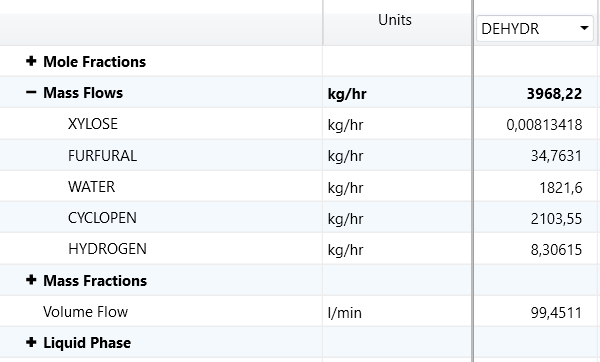
\includegraphics[width=.9\linewidth]{Παράρτημα/2023-01-13_18-10-03_screenshot.png}
\caption{Ρεύμα εξόδου από τον αντιδραστήρα R-CYCL για την παραγωγή της κυκλοπεντανόνης}
\end{figure}

\begin{figure}[htbp]
\centering
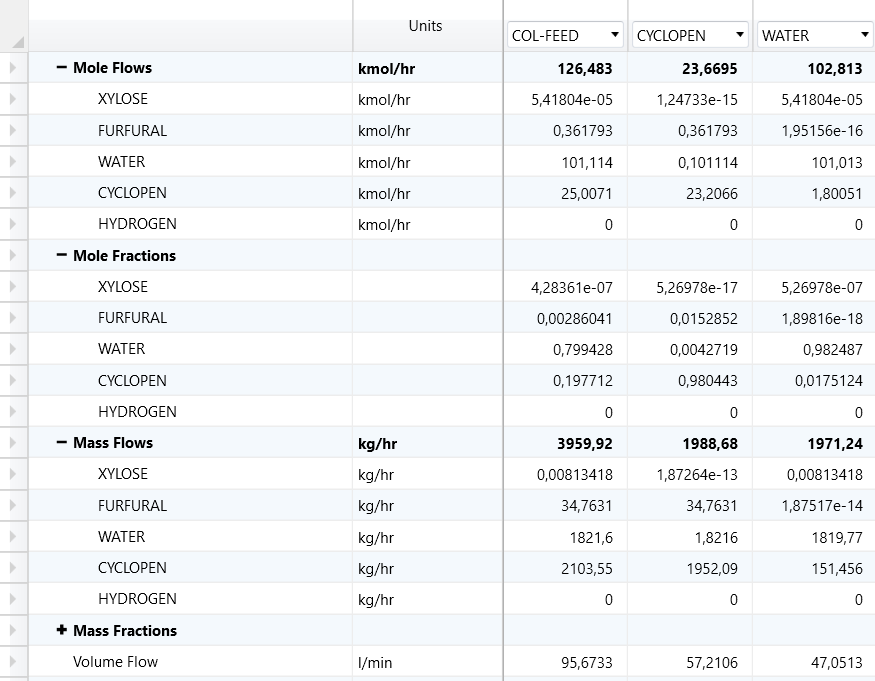
\includegraphics[width=.9\linewidth]{Παράρτημα/2023-01-13_18-10-10_screenshot.png}
\caption{Αποτελέσματα Αποστακτικής Στήλης}
\end{figure}

\begin{figure}[htbp]
\centering
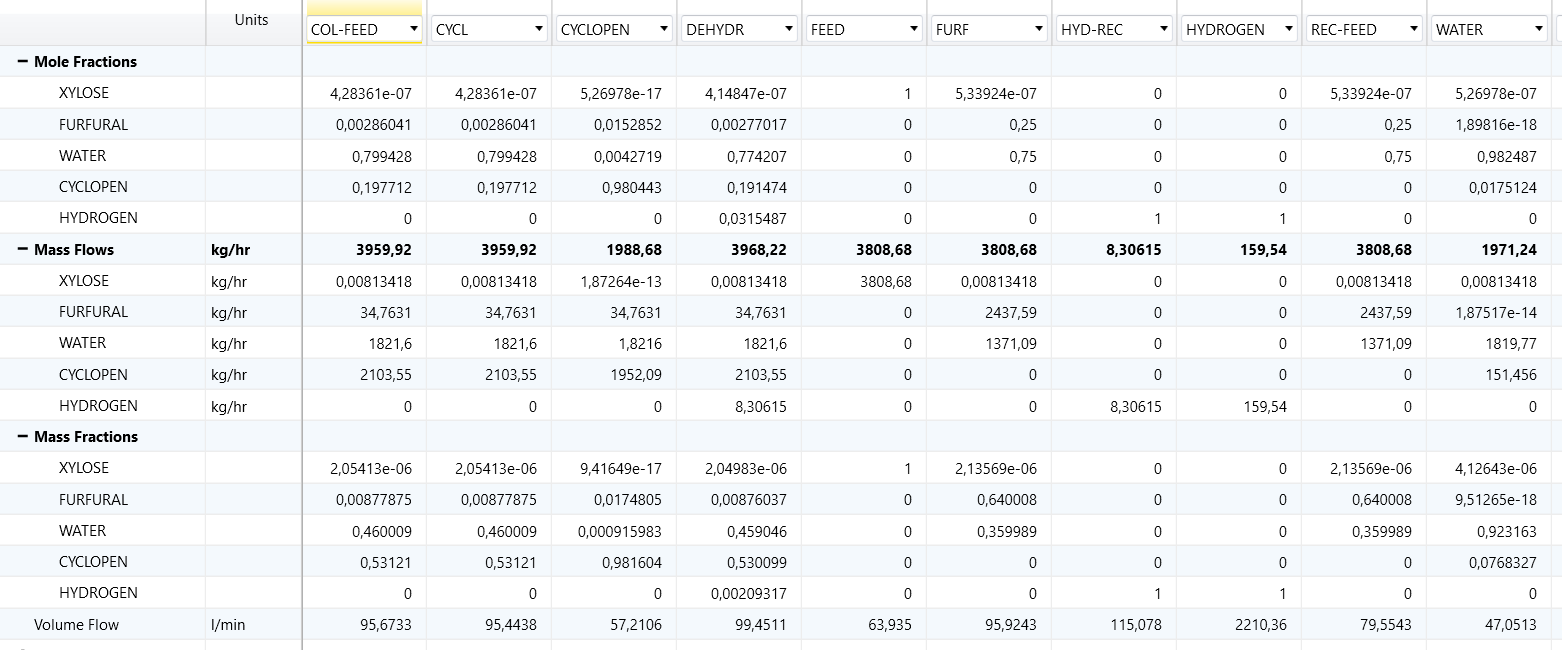
\includegraphics[width=.9\linewidth]{Παράρτημα/2023-01-13_18-10-19_screenshot.png}
\caption{Αποτελέσματα συνολικής διεργασίας για την κυκλοπεντανόνη}
\end{figure}

\pagebreak

\section{Παράρτημα ΣΤ - Github}
\label{sec:orgd9056cc}
Όλα τα αρχεία που έχουμε χρησιμοποιήσει κατά την διάρκεια του εξαμήνου είναι ανεβασμένα στο \href{https://github.com/Vidianos-Giannitsis/Process-Design}{Github μας}. Στο top level είναι μερικά γενικά αρχεία που έχουν χρειαστεί σε διάφορα των προσομοιώσεων. Στο φάκελο Diagrams υπάρχουν διαγράμματα ροής της διεργασίας σε διάφορα της στάδια τα οποία έχουν γίνει ως svgs στο Inkscape αλλά υπάρχουν και σε μορφή pdf. Στο φάκελο Calculations υπάρχουν διάφορα αρχεία Excel και Matlab τα οποία έχουν χρησιμοποιηθεί για ορισμένους υπολογισμούς. Ιδιαίτερα αυτούς που παρουσιάζονται στα άλλα παραρτήματα οι οποίοι είχαν αρκετή δουλειά. Υπάρχουν archived τα αρχεία που χρειαστήκαμε για όλες τις πρόοδους σε ξεχωριστούς φακέλους καθώς και τα αρχεία που χρειάστηκαν για την προετοιμασία της έκθεσης αυτής.

Τέλος, στον φάκελο Aspen υπάρχουν όλες οι προσομοιώσεις που έγιναν στο Aspen Plus για την εργασία, με ορισμένες να συνοδεύονται από documentation σε org format (αντίστοιχο του Markdown). Υπάρχουν τα 3 αρχεία προσομοιώσεων που σας στάλθηκαν μαζί με την εργασία καθώς και πολλά άλλα που είναι σε πιό πρώιμα στάδια.
\end{document}